\RequirePackage{etex}                 % ensure e-TeX extras available early
\providecommand\reserveinserts[1]{}   % safe no-op if class calls it
\documentclass[AMA,Times1COL]{WileyNJDv5} % note the hyphen in the class name

\articletype{Article Type}%

\received{Date Month Year}
\revised{Date Month Year}
\accepted{Date Month Year}
\journal{Journal}
\volume{00}
\copyyear{2023}
\startpage{1}

\raggedbottom

% ---------- Packages (kept lean and class-friendly) ----------
\usepackage{amsmath,amssymb}   % math
\usepackage{graphicx}          % figures
\usepackage{booktabs}          % tables
\usepackage{algorithm}         % algorithm float
\usepackage{algpseudocode}  
\usepackage{listings}          % code listings (ensure no local listings.sty)
\usepackage{enumitem}          % compact lists
\usepackage{rotating}          % sidewaysfigure/sidewaystable

% -------------------------------------------------------------

\begin{document}

\title{Edge-Optimized Hybrid Transformer Networks with Context-Aware Adaptation for Threat Classification in Visual Security Systems}

\author[1]{Anbi Tibina}
\author[2]{Dr. G. Naveen Sundar}
\author[3]{Dr. D. Narmadha}
\author[4]{Dr. S. Shirly}
\author[5]{Dr. Rosario Gilmary}
\author[6]{Adeyemi Abel Ajibesin}




\address[1]{\orgdiv{Division of Computer Science
and Engineering}, \orgname{Karunya Institute of Technology and Sciences}, \orgaddress{\state{Coimbatore}, \country{India}}}
\address[2]{\orgdiv{Division of Computer Science and Engineering}, \orgname{Karunya Institute of Technology and Sciences}, \orgaddress{\state{Coimbatore}, \country{India}}}
\address[3]{\orgdiv{Division of AIML}, \orgname{Karunya Institute of Technology and Sciences}, \orgaddress{\state{Coimbatore}, \country{India}}}
\address[4]{\orgdiv{Division of Computer Science and Engineering}, \orgname{Karunya Institute of Technology and Sciences}, \orgaddress{\state{Coimbatore}, \country{India}}}
\address[5]{\orgname{IFET College of Engineering}, \orgaddress{\state{Villupuram}, \country{India}}}
\address[6]{\orgdiv{Information Technology, Faculty Of Informatics And Design}, \orgname{Cape Peninsula University Of Technology}, \orgaddress{\state{Cape Town}, \country{South Africa}}}

\corres{Corresponding author Adeyemi Abel Ajibesin. \email{ajibesina@cput.ac.za}}


%\fundingInfo{Text}
%\JELinfo{ejlje}

\abstract[Abstract]{Visual security systems increasingly rely on automated video analytics to detect threats in real time under constrained compute and bandwidth. Effective models must balance recognition quality, robustness, and reliable confidence for alarm-driven decision making. A central challenge is that surveillance footage is noisy and context dependent, so similar motion patterns can represent benign activity or genuine violence depending on scene conditions. Conventional approaches such as three-dimensional convolutional neural networks (3D-CNNs) and large video transformers often trade accuracy for high computational cost, and their probability outputs can be poorly calibrated for threshold-based alerting. This work proposes an Edge-Optimized Hybrid Transformer Network with Context-Aware Adaptation (EO-HTN), combining a lightweight convolutional stem with a compact transformer stack and scene-conditioned temporal gating for efficient spatiotemporal reasoning. Experiments use two public benchmarks, Real-World Fight 2000 (RWF-2000) for binary violence detection and the University of Central Florida Crime (UCF-Crime) dataset for multi-class threat recognition under a clip-level protocol. EO-HTN achieves 93.4\% accuracy and 93.4\% F1-score on RWF-2000, and 86.3\% Top-1 accuracy with 83.2\% Macro F1-score on UCF-Crime, exceeding Video Swin Transformer Tiny (Video Swin-T) while using only 7.4 million parameters. Calibration improves on RWF-2000 with a Brier score of 0.078 and an Expected Calibration Error (ECE) of 3.2\%, supporting more trustworthy confidence estimates. These results suggest that EO-HTN is a practical foundation for edge-deployable threat analytics in surveillance pipelines.}

\keywords{Visual security systems; Threat classification; Edge AI; Hybrid transformer; Context-aware adaptation; Video violence detection; Calibration}

\jnlcitation{\cname{%
\author{Anbi Tibina}
\author{Dr. G. Naveen Sundar}
\author{Dr. D. Narmadha}
\author{Dr. S. Shirly}
\author{Dr. Rosario Gilmary}
\author{Adeyemi Abel Ajibesin}}.
\ctitle{On simplifying ‘incremental remap’-based transport schemes.} \cjournal{\it J Comput Phys.} \cvol{2021;00(00):1--18}.}

\maketitle

\renewcommand\thefootnote{}
\footnotetext{\textbf{Abbreviations:}  3D-CNNs, Three-dimensional Convolutional neural networks; EO-HTN, Edge-Optimized Hybrid Transformer Network; RWF-2000, Real-World Fight 2000; UCF-Crime, University of Central Florida Crime; Video Swin-T, Video Swin Transformer Tiny; ECE, Expected Calibration Error.}
\renewcommand\thefootnote{\fnsymbol{footnote}}
\setcounter{footnote}{1}

\section{Introduction}

Video surveillance has become a core sensing layer for public safety and industrial security, spanning transportation hubs, campuses, healthcare facilities, retail premises, and critical infrastructure. Modern deployments increasingly demand automatic threat understanding rather than simple recording, because human monitoring does not scale with the number of cameras and often suffers from fatigue and delayed response \cite{b1}. Practical video analytics therefore prioritizes fast, consistent recognition of violent and anomalous activities, together with confidence estimates that can support alarm ranking and operator triage.

A recurring obstacle in threat classification is the strong dependence of surveillance cues on local context. The same body motion or trajectory can reflect ordinary social contact, routine crowd flow, or intentional aggression once viewpoint, partial occlusion, and scene meaning are taken into account \cite{b2}. In practice, this interpretability problem is compounded by capture conditions that degrade evidence. Low illumination, motion blur, compression artifacts, and inconsistent camera placement can remove precisely the details that help separate intent, which increases the likelihood that a model escalates benign activity in dense scenes or overlooks subtle threats when key cues are hidden \cite{b3}.

A second limitation concerns the gap between how systems are evaluated in research settings and how they are used in deployments. Many security benchmarks use long, untrimmed videos where the threat-relevant interval is brief, so training labels and reported scores can shift depending on clip sampling and which segments receive supervision. Decision-making in control rooms is also governed by thresholds and escalation protocols, which makes probability quality important alongside accuracy \cite{b4}. Overconfident errors can create false alarms that drain operator attention and resources, while weak confidence on correct detections can slow intervention when timing matters most.

Conventional methods for threat recognition have primarily relied on three-dimensional convolutional neural networks (3D-CNNs) and two-stream designs that fuse spatial and temporal cues. Architectures such as Convolutional 3D (C3D), Inflated 3D ConvNet (I3D), and SlowFast have demonstrated strong performance by learning motion-sensitive representations, yet they can be computationally intensive and may not meet real-time constraints on edge devices \cite{b5}. When deployed in bandwidth-limited sites, these models can also impose high energy cost and memory pressure, which complicates multi-camera scaling.

More recent video transformers model long-range dependencies through self-attention and often improve recognition on large benchmarks. However, transformer-heavy models typically require high compute and memory bandwidth, and their performance can be sensitive to domain shift when backgrounds and camera viewpoints differ from training data. Moreover, large-capacity architectures do not automatically guarantee reliable confidence estimates, which limits their suitability for alerting systems that require calibrated probabilities for safe threshold selection.

This work proposes an Edge-Optimized Hybrid Transformer Network with Context-Aware Adaptation (EO-HTN) for threat classification in visual security systems. The proposed design couples a lightweight convolutional front-end, used to extract reliable local cues at low cost, with a compact transformer module that models spatiotemporal relations over short video clips. To account for scene variability, a context-aware adaptation unit summarizes the surrounding scene information and applies temporal gating so that feature responses are adjusted to prevailing conditions. This is intended to limit errors driven by background correlations and by motion patterns that appear similar across different activities. Overall, the architecture is built to sustain a usable trade-off between recognition quality, robustness under real capture noise, and feasibility on resource-limited devices, including support for post-training quantization to enable efficient inference.

The main contributions are summarized as follows:

\begin{itemize}
  \item A compact hybrid architecture, EO-HTN, that integrates efficient convolutional feature extraction with reduced-dimension self-attention for clip-level threat reasoning under edge constraints.
  \item A context-aware adaptation module based on scene token aggregation and temporal context gating to improve discrimination in ambiguous surveillance scenes.
  \item A comprehensive evaluation protocol on two public benchmarks, Real-World Fight 2000 (RWF-2000) for binary violence detection and University of Central Florida Crime (UCF-Crime) for multi-class threat classification, including ablation, cross-dataset transfer, and robustness under degradations.
  \item An edge-focused analysis that reports model size, latency, and throughput under floating-point 32-bit (FP32) and integer 8-bit (INT8) settings, together with reliability assessment through calibration metrics.
\end{itemize}

The remainder of this paper is organized as follows. Section~2 reviews related work on video-based threat recognition, efficient spatiotemporal modeling, and edge-oriented deployment strategies. Section~3 details the proposed Edge-Optimized Hybrid Transformer Network with Context-Aware Adaptation (EO-HTN), including the architectural design and learning objective. Section~4 describes the datasets, experimental protocol, model and training configuration, and reports the quantitative results with ablation, robustness, generalization, and calibration analyses, together with edge deployment measurements. Section~5 discusses the practical implications of the findings, highlights limitations observed in the experiments, and outlines directions for future improvement. Section~6 concludes the paper.



\section{Related Work}
\paragraph{Deep Learning Architectures for Video Anomaly and Violence Detection}
Deep learning based video anomaly detection in surveillance is often built around two competing needs. The model must capture temporal dependencies that reveal abnormal events, and it must remain reliable under shifts in scene layout, crowd density, lighting, and camera motion. Many recent methods address this tension through CNN backbones paired with recurrent units, memory modules, or multi-branch spatiotemporal designs, each introducing its own trade-offs in efficiency and transferability.

Pan \textit{et al.} \cite{b6} introduce a cross-scale spatiotemporal memory-augmented model for unsupervised anomaly detection and report very high AUC on UCSD Ped1/2, CUHK Avenue, and ShanghaiTech. The memory mechanism helps preserve prototypes of normal behavior and highlight deviations at inference, but it can be less reliable when test scenes exhibit unseen motion patterns and it adds a memory footprint that is not ideal for edge deployment. Singh and Pant \cite{b7} study few-shot anomaly detection in five-shot and ten-shot settings and achieve AUC above 90\%. Their results indicate that limited supervision can work when anomaly categories are constrained, while scaling to broader and overlapping classes remains challenging. Fatima and Ahmed \cite{b8} focus on real-time crime and violence detection by combining YOLOv8 with face recognition and report around 93\% performance. This object-centric design is useful when anomalies are tied to detectable entities, but it can miss cases where abnormality is mainly temporal, such as escalation or interaction dynamics. Ramoliya and Ganatra \cite{b9} combine ResNet50 with BiLSTM and report strong accuracy on UCF-Crime and ShanghaiTech, supporting the effectiveness of CNN features with recurrent temporal aggregation. The limitation is higher latency from sequential processing. Quirumbay Yagual \textit{et al.} \cite{b10} propose a CNN-GRU framework for early abnormal activity detection with high F1 on a custom surveillance setting, but domain bias can reduce transfer across camera views and scene statistics. Getsopon \textit{et al.} \cite{b11} integrate 2D and 3D CNN pathways and obtain very high accuracy on Hockey Fight and Violent Flows, showing that local spatiotemporal kernels capture short violence patterns effectively. However, low-light and visually degraded conditions remain less covered in many benchmarks. Sriveni and Loganathan \cite{b12} report very high accuracy using an active-learning-assisted deep ensemble, but the increased compute and parameter cost can conflict with edge constraints. Qi \textit{et al.} \cite{b13} present a real-time fistfight monitoring system with temporal localization and strong results on RWF-2000 and SCFD, though transformer backbones typically increase training and inference cost. Manju \textit{et al.} \cite{b14} combine Mask R-CNN with LSTM and show competitive performance on UCF-Crime and CUHK, but occlusion can disrupt region extraction and downstream temporal modeling.


\paragraph{Transformer and Attention-Based Hybrid Models}
Recent work increasingly relies on transformers and attention to capture long-range spatiotemporal dependencies that are difficult to model with purely convolutional or recurrent backbones. CrossTrans-Surv by Reddy \cite{b15} uses multimodal cross-attention to fuse RGB and LiDAR cues, reporting improved robustness under challenging lighting. The core benefit comes from complementary sensing, but the requirement for multiple synchronized sensors limits applicability in typical CCTV deployments where only RGB streams are available. Wang \textit{et al.} \cite{b16} present a hybrid Transformer--CNN with explicit context encoding for violence detection and report strong results on RWF-2000. The design highlights lightweight convolution's role in but morphing local motion evidence and attention in perfecting global interactions. A major problem here is the transformer components may fit too well to the training clips if they are of short length or if the background effect (bias) is strong, which can negatively affect the inter-scene robustness. Mao \textit{et al.}\cite{b17} suggest hierarchical temporal excitation to enhance the violence recognition through temporal reasoning and they achieve the highest accuracies on the MCV and HockeyFight datasets. The method demonstrates that multi-level temporal emphasis can improve recognition of subtle transitions, yet the higher compute cost makes it harder to translate these gains to edge settings without careful compression or approximation. Khaled \textit{et al.} \cite{b18} combine TimeSformer with multiple-instance learning to recognize anomalous activities on a UCF-Crime subset and report performance above 90\%. The MIL formulation is useful for untrimmed surveillance because it reduces the need for precise clip boundaries, but the approach typically benefits from segment-level supervision or reliable bag construction, which can still create annotation overhead. Habeb \textit{et al.} \cite{b19} introduce an attention-based unsupervised anomaly detection framework evaluated on ShanghaiTech and CUHK with strong AUC. Unsupervised attention can surface irregular motion patterns without labels, but generalization remains sensitive to video quality. Compression artifacts, low illumination, and camera jitter can shift the normal pattern distribution and increase false alarms. Zhang \textit{et al.} \cite{b20} explore a 3D CNN plus transformer framework for behavior recognition and report high accuracy on public datasets, supporting the view that convolutions capture short-range motion while transformers model broader temporal relations. A missing piece is consistent reporting of real-time throughput and latency, which is important for surveillance systems that must operate under strict compute budgets. Domain-specific transformer designs have also been studied. Ji \textit{et al.} \cite{b21} propose a dual transformer model for passenger anomaly detection in elevator cabs and achieve high accuracy in that constrained environment, but the specialization can limit generalization when viewpoints, crowd density, and scene context change. Dongping \textit{et al.} \cite{b22} enhance temporal modeling through multi-channel coupling and report strong performance on violence datasets, yet the lack of real-time benchmarking makes it difficult to judge deployment feasibility. Overall, these studies suggest that attention mechanisms improve spatiotemporal reasoning, especially in complex interactions and long-range dependencies. At the same time, reliance on heavy transformer capacity, multimodal sensors, or additional supervision can limit practical adoption. This motivates compact hybrid designs that retain attention benefits while controlling compute, memory, and annotation burden.


\paragraph{Reviews, Frameworks, and Application Studies}
Beyond model-centric contributions, several studies emphasize deployable frameworks, system integration, and broader syntheses of the surveillance anomaly literature. Flores-Monroy \textit{et al.} \cite{b23} propose an online modular pipeline that combines anomaly detection with multiclass classification and report clip-level performance on UCF-Crime. The modular design is attractive for engineering because components can be swapped or upgraded independently. However, decoupling modules can weaken end-to-end coherence, since detection errors propagate to classification without joint optimization. System-oriented implementations often aim for practical suspicious-activity monitoring under real constraints. Wani and Faridi \cite{b24} present a deep-learning-based surveillance system and report high accuracy across public and custom data. Their use of LRCN-style temporal modeling aligns with common deployment practice, but such recurrent pipelines can be less robust when motion is irregular, occlusions are frequent, or clip boundaries are noisy. In a similar applied direction, Reddy \textit{et al.} \cite{b25} discuss smart surveillance for violence detection in real-time CCTV scenarios and report strong outcomes. A recurring limitation in such application studies is incomplete quantitative reporting across standard benchmarks, which makes reproducibility and fair comparison difficult. Survey and overview papers provide useful mapping of the design space but often stop short of evidence-based benchmarking. Chen \cite{b26} reviews deep-learning-driven behavior analysis across datasets and highlights the role of representation learning in surveillance. The work is mainly conceptual and offers limited quantitative synthesis, so the relative tradeoffs between accuracy, latency, and robustness remain underspecified. Kolaib and Waleed \cite{b27} provide a focused investigation of deep-learning crime detection systems and organize common model families. Since the study is comparative rather than experimental, it cannot validate conclusions under controlled settings. Gupta and Tyagi \cite{b28} similarly compile a comprehensive review of anomaly detection advances and summarize trends across methods, but the absence of new experiments means that claims about generalization and deployment cost still rely on reported results rather than standardized re-evaluation. Some contributions revisit classic feature engineering either as stand-alone solutions or as baselines. Rajput \cite{b29} evaluates anomaly detection using LPQ ensembles, SP-HOG, STAP, and statistical descriptors and reports strong performance on UCSD and CUHK. These approaches can be interpretable and lightweight, but their representational ceiling is typically lower than modern deep models when scene variation increases, since handcrafted descriptors may not adapt to changing viewpoints and complex interactions. At the other extreme, Aldulimy and Alazzawi \cite{b30} propose a CNN-based violence prediction model with GAMMA correction and report very high accuracy on RLV. The dependence on illumination-oriented preprocessing can become a liability when lighting conditions shift in unexpected ways, since enhancement parameters may amplify noise or alter appearance statistics. Recent work also targets stronger temporal reasoning with attention while remaining application-relevant. Han \textit{et al.} \cite{b31} combine Temporal-CNN modeling with self-attention for violence recognition on RWF-2000 and report competitive performance. The main tradeoff is inference time, as attention layers and temporal stacks can add latency that is difficult to absorb on edge hardware without compression. Finally, Shen \textit{et al.} \cite{b32} explore inter-patch spatiotemporal relation prediction for anomaly detection and report strong results on UCSD and Avenue. Patch-level relation modeling can capture fine anomalies, but it often increases memory demand because many patch interactions must be stored or processed, which complicates deployment at scale. Taken together, these works show that practical surveillance research spans more than architecture design. Framework modularity, reporting rigor, and deployment constraints often determine whether strong offline accuracy translates into reliable on-site performance. These considerations motivate compact end-to-end pipelines that preserve temporal reasoning while controlling latency and memory use.


\section{System Methodology}
This section presents the end-to-end methodology for threat classification in visual security systems using the proposed Edge-Optimized Hybrid Transformer Network with Context-Aware Adaptation (EO-HTN). The pipeline follows a clip-based recognition protocol, combining lightweight spatial encoding with compact temporal attention and context-aware feature modulation for edge-ready inference, as illustrated in Fig.~\ref{fig:eohtn_arch}.

\begin{figure}[!t]
\centering
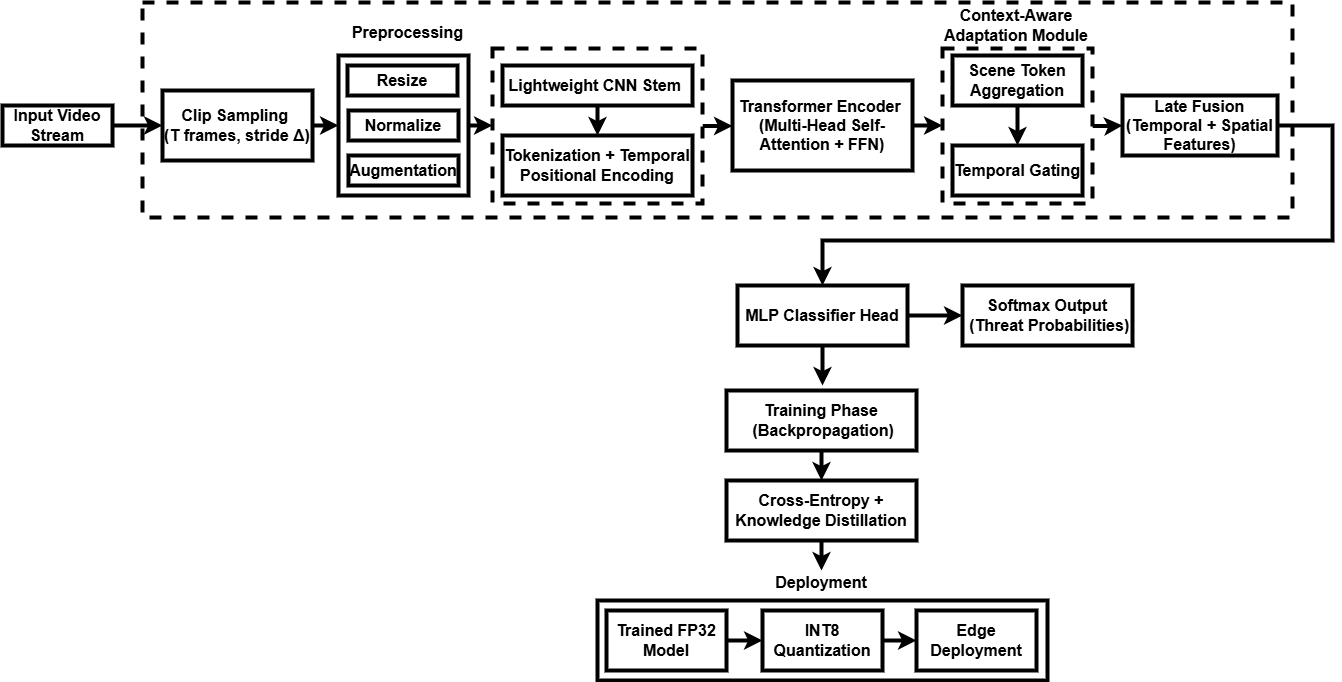
\includegraphics[width=0.9\linewidth]{1.drawio.png}
\caption{Architecture of the proposed EO-HTN framework.}
\label{fig:eohtn_arch}
\end{figure}


\subsection{Problem Formulation}
Threat classification is formulated as supervised video recognition over short clips extracted from surveillance streams. Let $\mathcal{D}=\{(\mathbf{X}_i, y_i)\}_{i=1}^{N}$ denote a labeled dataset, where $\mathbf{X}_i \in \mathbb{R}^{T\times H \times W \times 3}$ is a clip of $T$ RGB frames resized to $H \times W$, and $y_i \in \{1,\dots,C\}$ is the threat class label. The proposed Edge-Optimized Hybrid Transformer Network with Context-Aware Adaptation (EO-HTN) is parameterized by $\theta$ and outputs a class distribution $\hat{\mathbf{p}}_i \in [0,1]^C$ using the softmax mapping in Eq.~(\ref{eq:softmax_out}). In deployment, the output vector $\hat{\mathbf{p}}_i$ is interpreted as a risk profile over threat types, where the predicted class is $\arg\max_c \hat{p}_{i,c}$ and the largest probability can be used for alarm thresholding. The use of softmax in Eq.~(\ref{eq:softmax_out}) also enables confidence-aware evaluation beyond Top-1 accuracy, since probability mass assigned to confusable classes reflects uncertainty that is common in surveillance footage.

\begin{equation}
\hat{\mathbf{p}}_i = \mathrm{softmax}\!\left(\mathbf{z}_i\right), \qquad 
\mathrm{softmax}(\mathbf{z})_c = \frac{\exp(z_c)}{\sum_{k=1}^{C}\exp(z_k)} .
\label{eq:softmax_out}
\end{equation}

\subsection{Clip Construction and Preprocessing}
Each clip is sampled from a source video using a fixed temporal length $T$ and stride $\Delta$. If $\mathbf{I}_t$ is the $t$-th raw frame in the video, the clip tensor $\mathbf{X}$ is constructed by Eq.~(\ref{eq:clip_sampling}), followed by resizing and normalization. The sampling strategy in Eq.~(\ref{eq:clip_sampling}) converts an untrimmed stream into a sequence of short, fixed-length decision units, which is compatible with edge inference where buffering long segments increases latency and memory use. The parameters $T$ and $\Delta$ control the effective temporal coverage. Smaller $\Delta$ emphasizes fine motion continuity, while larger $\Delta$ increases temporal span and can better capture delayed cues such as escalation patterns. After sampling, each frame is resized to $(H,W)$ to standardize compute, and normalization is applied to reduce sensitivity to illumination and camera-specific color response. These steps ensure that the learning objective focuses on spatiotemporal structure rather than raw intensity scale.

\begin{equation}
\mathbf{X} = \big[\mathbf{I}_{t_0}, \mathbf{I}_{t_0+\Delta}, \dots, \mathbf{I}_{t_0+(T-1)\Delta}\big] .
\label{eq:clip_sampling}
\end{equation}

\subsection{Lightweight Convolutional Stem}
EO-HTN begins with a compute-efficient convolutional stem that extracts local spatial features from each frame. Depthwise-separable convolution is used to reduce parameter count and memory access cost. For an input feature map $\mathbf{U}\in\mathbb{R}^{H\times W\times C_{\mathrm{in}}}$, the depthwise step applies a channel-wise spatial kernel, and the pointwise step mixes channels. The two-stage operation is summarized in Eq.~(\ref{eq:dsconv}). From a theoretical standpoint, $\mathrm{DW}(\cdot)$ can be viewed as learning channel-specific spatial detectors that respond to edges, textures, and small object parts, while $\mathrm{PW}(\cdot)$ learns cross-channel combinations that form higher-level descriptors. This separation is particularly valuable in surveillance scenes because the visual evidence for threats can be local and sparse, such as a raised arm, a sudden collision, or a small region of smoke. In addition, the stem acts as an inductive bias for locality, complementing the transformer which is more flexible but can be more expensive without careful design.

The stem outputs a compact feature tensor $\mathbf{F}\in\mathbb{R}^{T\times h \times w \times d}$, where $(h,w)$ are the spatial dimensions after downsampling and $d$ is the embedding width used by the transformer. Reducing the spatial map early limits the token count that reaches self-attention, which directly improves efficiency because the attention cost grows with the number of tokens. This design also helps regularize the model because excessively fine spatial grids can encourage learning camera-specific details that do not transfer across sites.

\begin{equation}
\mathbf{V} = \mathrm{PW}\!\left(\mathrm{DW}(\mathbf{U})\right),
\label{eq:dsconv}
\end{equation}

\subsection{Tokenization and Temporal Positional Encoding}
The spatial grid $(h\times w)$ at each time step is flattened into a token sequence. Let $\mathbf{f}_t \in \mathbb{R}^{(hw)\times d}$ denote the tokens at time $t$. Temporal order is injected through learnable temporal positional embeddings $\mathbf{E}\in\mathbb{R}^{T\times d}$ added to all tokens at the same time index. The token sequence $\mathbf{H}^{(0)}$ is formed by Eq.~(\ref{eq:token_pos}), where $L=T\cdot hw$. This construction imposes a structured token layout in which contiguous segments correspond to the same time index. The learnable embeddings $\mathbf{E}_t$ serve as a time stamp, allowing attention layers to distinguish whether two spatial tokens originate from the same frame or different frames, even when their visual content is similar.

The temporal encoding in Eq.~(\ref{eq:token_pos}) is especially important for clips sampled from untrimmed videos, where multiple clips may share similar backgrounds but differ in action dynamics. Without temporal position, self-attention can become permutation-invariant across frames, which undermines the representation of motion direction and event ordering. Learnable temporal embeddings are also compatible with edge deployment because they add negligible compute and can adapt to the clip sampling policy during training.

\begin{equation}
\mathbf{H}^{(0)} = \mathrm{concat}\Big(\mathbf{f}_1+\mathbf{E}_1,\dots,\mathbf{f}_T+\mathbf{E}_T\Big) \in \mathbb{R}^{L\times d},
\label{eq:token_pos}
\end{equation}

\subsection{Compact Transformer Encoder with Efficient Self-Attention}
The transformer encoder refines the token sequence using multi-head self-attention (MHSA) and a feed-forward network (FFN). Attention provides an adaptive mixing mechanism, where each token can integrate evidence from spatial regions and time steps that are most informative for the current clip. For head dimension $d_h=d/M$ with $M$ heads, the scaled dot-product attention is defined by Eq.~(\ref{eq:attn_core}). The normalization factor $\sqrt{d_h}$ in Eq.~(\ref{eq:attn_core}) stabilizes gradients by preventing the dot products $\mathbf{Q}\mathbf{K}^\top$ from growing too large as dimensionality increases, which is relevant for consistent optimization when clip content varies substantially.

\begin{equation}
\mathrm{Attn}(\mathbf{Q},\mathbf{K},\mathbf{V}) = 
\mathrm{softmax}\!\left(\frac{\mathbf{Q}\mathbf{K}^{\top}}{\sqrt{d_h}}\right)\mathbf{V},
\label{eq:attn_core}
\end{equation}

MHSA in Eq.~(\ref{eq:mhsa}) uses multiple heads so that different subspaces can specialize. In surveillance clips, one head may focus on rapid motion regions, another may track human interaction zones, and another may attend to contextual cues such as fire, smoke, or sudden crowd dispersion. The reduced embedding dimension and limited transformer depth keep the attention computation practical, while still enabling cross-frame dependency modeling that is difficult for purely convolutional backbones.

\begin{equation}
\mathrm{MHSA}(\mathbf{H}) = \mathrm{concat}\!\left(\mathrm{Attn}(\mathbf{H}\mathbf{W}^Q_m,\mathbf{H}\mathbf{W}^K_m,\mathbf{H}\mathbf{W}^V_m)\right)_{m=1}^{M}\mathbf{W}^O .
\label{eq:mhsa}
\end{equation}

A transformer block updates tokens via residual connections as shown in Eq.~(\ref{eq:trans_block}), where $\mathrm{LN}(\cdot)$ is layer normalization. The nested residual structure in Eq.~(\ref{eq:trans_block}) has a practical role beyond standard transformer design. It encourages the network to learn refinements relative to the incoming representation rather than rewriting it entirely, which is helpful when many surveillance frames contain redundant background content. The FFN expands and contracts feature dimensions internally, allowing non-linear reweighting of token channels after attention has mixed information across tokens. This combination supports a two-step reasoning pattern, where attention selects relevant evidence and the FFN reshapes it into class-discriminative directions.

The refinement in Eq.~(\ref{eq:trans_block}) supports context aggregation across time and across spatial regions without resorting to heavy transformer capacity. In particular, the attention mechanism can connect semantically related regions that are separated in space and time, such as a hand movement followed by a reaction, or a flash followed by smoke. Keeping the number of layers small reduces the risk of overfitting to camera-specific patterns and maintains an edge-friendly compute profile. The internal structure of the proposed compact transformer encoder is illustrated in Fig.~\ref{fig:compact_transformer_encoder}.

\begin{equation}
\mathbf{H}^{(\ell+1)} = \mathbf{H}^{(\ell)} + \mathrm{FFN}\!\Big(\mathrm{LN}\big(\mathbf{H}^{(\ell)} + \mathrm{MHSA}(\mathrm{LN}(\mathbf{H}^{(\ell)}))\big)\Big).
\label{eq:trans_block}
\end{equation}

\begin{figure}[!t]
  \centering
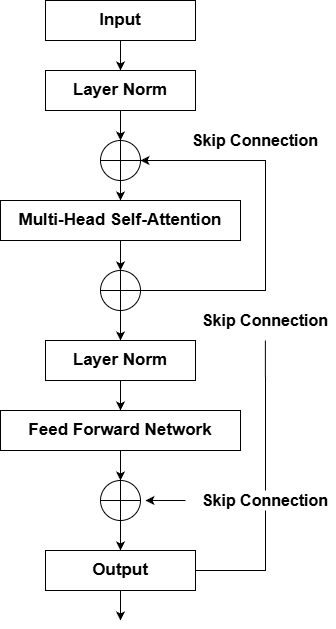
\includegraphics[height=10cm, width=8cm]{2.drawio.png}
  \caption{Architecture of the compact transformer encoder block.}
  \label{fig:compact_transformer_encoder}
\end{figure}



\subsection{Context-Aware Adaptation via Scene Token Aggregation and Temporal Gating}
Surveillance scenes differ in viewpoint, crowd density, and background motion, and these factors can distort threat cues. EO-HTN introduces a context-aware adaptation module that produces a scene descriptor and uses it to gate temporal features. First, a scene token $\mathbf{s}\in\mathbb{R}^{d}$ is computed by averaging all tokens, as defined in Eq.~(\ref{eq:scene_token}).
\begin{equation}
\mathbf{s} = \frac{1}{L}\sum_{j=1}^{L}\mathbf{H}^{(L_{\mathrm{tr}})}_j ,
\label{eq:scene_token}
\end{equation}
where $\mathbf{H}^{(L_{\mathrm{tr}})}$ denotes the output of the final transformer layer and $\mathbf{H}^{(L_{\mathrm{tr}})}_j$ is the $j$-th token. Next, a per-time summary $\bar{\mathbf{h}}_t$ is obtained by averaging spatial tokens at time $t$, and a gating vector $\mathbf{g}_t$ is produced by Eq.~(\ref{eq:gating}).
\begin{equation}
\bar{\mathbf{h}}_t = \frac{1}{hw}\sum_{u=1}^{hw}\mathbf{h}_{t,u}, \qquad
\mathbf{g}_t = \sigma\!\left(\mathbf{W}_g[\bar{\mathbf{h}}_t;\mathbf{s}] + \mathbf{b}_g\right),
\label{eq:gating}
\end{equation}
where $\sigma(\cdot)$ is the sigmoid function and $[\cdot;\cdot]$ denotes concatenation. The gated temporal representation $\tilde{\mathbf{h}}_t$ is then computed by Eq.~(\ref{eq:gated_feat}).
\begin{equation}
\tilde{\mathbf{h}}_t = \mathbf{g}_t \odot \bar{\mathbf{h}}_t ,
\label{eq:gated_feat}
\end{equation}
where $\odot$ denotes element-wise multiplication. The gating in Eq.~(\ref{eq:gated_feat}) suppresses context-induced activations that are inconsistent with the global scene descriptor in Eq.~(\ref{eq:scene_token}).

\subsection{Late Fusion and Classification Head}
EO-HTN combines spatial and temporal evidence through late fusion. A temporal feature $\mathbf{u}\in\mathbb{R}^{d}$ is formed by averaging the gated summaries, and a spatial feature $\mathbf{v}\in\mathbb{R}^{d}$ is formed by pooling tokens. The fused representation $\mathbf{r}$ is defined by Eq.~(\ref{eq:fusion}).
\begin{equation}
\mathbf{u} = \frac{1}{T}\sum_{t=1}^{T}\tilde{\mathbf{h}}_t, \qquad
\mathbf{v} = \frac{1}{L}\sum_{j=1}^{L}\mathbf{H}^{(L_{\mathrm{tr}})}_j, \qquad
\mathbf{r} = [\mathbf{u};\mathbf{v}] .
\label{eq:fusion}
\end{equation}
A two-layer multilayer perceptron (MLP) maps $\mathbf{r}$ to logits $\mathbf{z}$, as expressed in Eq.~(\ref{eq:mlp_logits}), and probabilities are then obtained using Eq.~(\ref{eq:softmax_out}).
\begin{equation}
\mathbf{z} = \mathbf{W}_2\,\phi(\mathbf{W}_1\mathbf{r}+\mathbf{b}_1)+\mathbf{b}_2,
\label{eq:mlp_logits}
\end{equation}
where $\phi(\cdot)$ is a non-linear activation function.


\subsection{Training Objective with Label Smoothing and Edge Distillation}
Training uses cross-entropy with label smoothing to reduce overconfident predictions under ambiguous surveillance cues. For smoothed target distribution $\mathbf{y}^{LS}$ and predicted probability $\hat{\mathbf{p}}$ from Eq.~(\ref{eq:softmax_out}), the loss is defined by Eq.~(\ref{eq:ce_ls}).
\begin{equation}
\mathcal{L}_{\mathrm{CE}} = -\sum_{c=1}^{C} y^{LS}_c \log(\hat{p}_c), \qquad
\mathbf{y}^{LS} = (1-\epsilon)\mathbf{y} + \frac{\epsilon}{C}\mathbf{1},
\label{eq:ce_ls}
\end{equation}
where $\epsilon$ is the smoothing factor and $\mathbf{1}$ is an all-ones vector. To improve edge behavior, knowledge distillation aligns student and teacher distributions at temperature $\tau$. The distillation term is computed by Eq.~(\ref{eq:kd}).
\begin{equation}
\mathcal{L}_{\mathrm{KD}} = \tau^2\,\mathrm{KL}\!\left(\mathrm{softmax}\!\left(\frac{\mathbf{z}^{(T)}}{\tau}\right)\;\middle\|\;\mathrm{softmax}\!\left(\frac{\mathbf{z}^{(S)}}{\tau}\right)\right),
\label{eq:kd}
\end{equation}
where $\mathbf{z}^{(T)}$ and $\mathbf{z}^{(S)}$ are teacher and student logits, and $\mathrm{KL}(\cdot\|\cdot)$ is the Kullback--Leibler divergence. The full objective combines Eq.~(\ref{eq:ce_ls}) and Eq.~(\ref{eq:kd}) as shown in Eq.~(\ref{eq:total_loss}).
\begin{equation}
\mathcal{L} = \mathcal{L}_{\mathrm{CE}} + \lambda\,\mathcal{L}_{\mathrm{KD}},
\label{eq:total_loss}
\end{equation}
where $\lambda$ controls the influence of distillation.

\subsection{INT8 Quantization for Edge Deployment}
To reduce memory footprint and improve throughput, post-training INT8 quantization maps floating-point weights to discrete levels using a scale factor. A standard symmetric quantization rule is expressed in Eq.~(\ref{eq:quant}).
\begin{equation}
\mathbf{W}_q = s\cdot \mathrm{clip}\!\left(\mathrm{round}\!\left(\frac{\mathbf{W}}{s}\right), -127, 127\right),
\label{eq:quant}
\end{equation}
where $\mathbf{W}$ is a floating-point weight tensor, $\mathbf{W}_q$ is its quantized counterpart, and $s$ is a per-tensor or per-channel scale. The mapping in Eq.~(\ref{eq:quant}) reduces storage and can accelerate inference on hardware with INT8 support.

\subsection{Pseudo-Algorithm}
Algorithm~\ref{alg:eohtn_train} summarizes the training procedure, referencing the key computations introduced in Eq.~(\ref{eq:clip_sampling})--Eq.~(\ref{eq:total_loss}). The same forward path is used during inference, with optional INT8 deployment governed by Eq.~(\ref{eq:quant}).

\begin{algorithm}[t]
\caption{Training procedure for EO-HTN}
\label{alg:eohtn_train}
\begin{algorithmic}[1]
\Require Dataset $\mathcal{D}$, epochs $E$, label smoothing $\epsilon$, distillation weight $\lambda$, temperature $\tau$
\State Initialize EO-HTN parameters $\theta$ and optimizer
\For{$epoch = 1$ to $E$}
  \ForAll{mini-batch $\mathcal{B}=\{(\mathbf{X}_i,y_i)\}$ from $\mathcal{D}$}
    \State Construct clips using Eq.~(\ref{eq:clip_sampling}) and preprocess inputs
    \State Extract stem features via depthwise-separable convolution in Eq.~(\ref{eq:dsconv})
    \State Tokenize and add temporal positional embeddings using Eq.~(\ref{eq:token_pos})
    \State Apply transformer blocks using Eq.~(\ref{eq:mhsa}) and Eq.~(\ref{eq:trans_block})
    \State Compute scene token and temporal gating using Eq.~(\ref{eq:scene_token}) to Eq.~(\ref{eq:gated_feat})
    \State Fuse features using Eq.~(\ref{eq:fusion}) and compute logits using Eq.~(\ref{eq:mlp_logits})
    \State Obtain probabilities using Eq.~(\ref{eq:softmax_out})
    \State Compute $\mathcal{L}_{\mathrm{CE}}$ with label smoothing using Eq.~(\ref{eq:ce_ls})
    \State Compute distillation loss $\mathcal{L}_{\mathrm{KD}}$ using Eq.~(\ref{eq:kd})
    \State Compute total loss $\mathcal{L}$ using Eq.~(\ref{eq:total_loss})
    \State Update $\theta$ by backpropagation
  \EndFor
\EndFor
\Statex \textbf{Optional:} Quantize weights for deployment using Eq.~(\ref{eq:quant})
\end{algorithmic}
\end{algorithm}





\section{RESULTS}
This section reports the empirical evaluation of EO-HTN on public surveillance benchmarks and summarizes its recognition accuracy, robustness, and deployment efficiency under practical operating constraints. Results are presented with controlled split protocols and complementary analyses, including ablations, cross-dataset transfer, degradation tests, and calibration behaviour.


\subsection{Datasets for Threat Classification in Visual Security Systems}
This study evaluates the proposed model on two public benchmarks that represent distinct operating conditions for visual security analytics. As summarized in Table~\ref{tab:datasets_threat}, RWF-2000 supports a clear binary decision setting where the model must separate violent activity from non-violent scenes using short surveillance clips. UCF-Crime is a more challenging benchmark because it is dominated by long, untrimmed recordings spanning many threat categories and filming conditions. Relevant events can be brief and dispersed within extended timelines, which forces the model to preserve temporal evidence over longer horizons while remaining stable under wide variation in scene layout, viewpoint, and background activity. When evaluated together with a short-clip violence dataset, the two benchmarks test complementary capabilities. One primarily rewards clear violence versus non-violence separation, while the other stresses multi-class threat recognition under realistic scene diversity and temporally sparse events.

RWF-2000 comprises 2{,}000 short CCTV-style clips annotated with two labels, \textit{Violence} and \textit{Non-Violence}. It is useful for assessing decision reliability in monitoring pipelines because the non-violent class often contains rapid motion, close interactions, and crowded movement that can visually resemble aggressive behavior. In our experiments, we use a standard split with 1{,}600 clips for training and 400 clips for testing. This setting preserves a meaningful held-out test set for reporting, while leaving sufficient training examples to learn robust spatiotemporal cues. Given the short duration of the clips, the model is encouraged to form discriminative evidence quickly, which is consistent with edge-oriented deployments where early and stable decisions are preferred.


UCF-Crime contains approximately 1{,}900 untrimmed videos spanning 13 anomaly or threat types, with many experimental protocols also including a Normal class in the evaluation setup. The untrimmed format increases difficulty because threat-relevant segments may occupy only a portion of the timeline, while the remaining frames may be visually benign. The dataset includes substantial variation in viewpoint, illumination, crowd density, and background activity. This makes UCF-Crime valuable for testing context-aware adaptation because the model must avoid overreacting to scene-specific nuisances while still responding to genuine threat signals. We follow the commonly used benchmark protocol splits reported in prior work, and train and evaluate using a clip-level protocol to ensure consistent supervision and comparable reporting.

The two datasets in Table~\ref{tab:datasets_threat} were selected to cover both ends of the threat recognition spectrum. RWF-2000 measures how well the model separates violence from non-violence when the input is short and the decision boundary is tight. UCF-Crime stresses generalization because threat categories span multiple contexts and the videos are long, which requires temporal consistency and resistance to background bias. This pairing allows us to examine not only classification performance, but also how design choices behave under different data regimes.

\begin{table}[t]
\centering
\caption{Datasets used for threat classification in visual security systems.}
\label{tab:datasets_threat}
\renewcommand{\arraystretch}{1.1}
\setlength{\tabcolsep}{3.5pt}
\resizebox{\linewidth}{!}{%
\begin{tabular}{|p{2.1cm}|p{3.0cm}|p{3.0cm}|p{2.2cm}|p{2.6cm}|p{4.0cm}|}
\hline
\textbf{Dataset} & \textbf{Primary Task} & \textbf{Threat Categories} & \textbf{Dataset Size} & \textbf{Data Split} & \textbf{Key Characteristics} \\
\hline
RWF-2000 & Violence / threat classification & 2 (Violence, Non-Violence) & 2{,}000 short clips & 1{,}600 Train / 400 Test & Real-world CCTV footage; widely used for violence detection; short clips support fast decisions. \\
\hline
UCF-Crime & Multi-class threat recognition & 13 threat types (plus Normal in many setups) & $\sim$1{,}900 untrimmed videos & Standard protocol splits & Diverse scenes and long temporal context; untrimmed videos increase difficulty; standard anomaly benchmark. \\
\hline
\end{tabular}%
}
\end{table}


\subsection{Dataset-wise Data Split Protocol}
To ensure that the reported performance reflects generalization rather than memorization, we define explicit training, validation, and test partitions for each benchmark. Table~\ref{tab:datasplit_threat} summarizes the adopted splits, including the number of samples and the guiding strategy used to form each subset. The validation subset is used for model selection, hyperparameter tuning, and early stopping, while the test subset is kept untouched until final reporting. This separation is important for surveillance data because clips often share similar backgrounds, camera viewpoints, or lighting conditions. A careful split reduces the risk that visually related content appears across partitions and inflates results. For RWF-2000, the dataset contains 2{,}000 surveillance clips with two classes. We allocate 1{,}400 clips (70\%) for training, 200 clips (10\%) for validation, and 400 clips (20\%) for testing, as shown in Table~\ref{tab:datasplit_threat}. The split is stratified so that the Violence and Non-Violence categories remain balanced across all partitions. This choice preserves the original class proportions during optimization and makes the validation signal stable. The 20\% held-out test portion is intentionally larger than a minimal split because binary violence classification can be sensitive to scene bias. A stronger test set provides a more reliable estimate of how the model behaves on unseen cameras and environments. For UCF-Crime, the benchmark comprises approximately 1{,}900 untrimmed videos spanning multiple threat types. We use a video-level split with 1{,}520 videos (80\%) for training, 190 videos (10\%) for validation, and 190 videos (10\%) for testing, as reported in Table~\ref{tab:datasplit_threat}. The video-level constraint means that clips extracted for clip-level training and evaluation come only from videos assigned to that partition. This avoids leakage where visually adjacent segments from the same original video might otherwise appear in both training and testing. Since UCF-Crime videos are long and contain substantial within-video redundancy, enforcing this constraint is essential for a fair assessment of multi-class threat recognition.



\begin{table}[t]
\centering
\caption{Dataset-wise data split used in experiments.}
\label{tab:data_split_threat}
\renewcommand{\arraystretch}{1.1}
\setlength{\tabcolsep}{3.5pt}
\resizebox{\linewidth}{!}{%
\begin{tabular}{|p{2.2cm}|p{2.2cm}|p{2.6cm}|p{2.6cm}|p{2.4cm}|p{5.0cm}|}
\hline
\textbf{Dataset} & \textbf{Total Samples} & \textbf{Training Set} & \textbf{Validation Set} & \textbf{Test Set} & \textbf{Split Strategy} \\
\hline
RWF-2000 & 2{,}000 clips & 1{,}400 (70\%) & 200 (10\%) & 400 (20\%) & Stratified split with balanced Violence and Non-Violence class proportions across all subsets. \\
\hline
UCF-Crime & $\sim$1{,}900 videos & 1{,}520 (80\%) & 190 (10\%) & 190 (10\%) & Video-level split to prevent leakage; clip-level training and evaluation are performed within each split using clips sampled from the assigned videos. \\
\hline
\end{tabular}%
}
\end{table}


\subsection{Model Configuration of EO-HTN}
The proposed Edge-Optimized Hybrid Transformer Network (EO-HTN) is designed to balance recognition performance with deployment practicality in resource-constrained visual security systems. The configuration choices in Table~\ref{tab:model_config_eohtn} reflect two constraints that often conflict in surveillance analytics. The model must retain enough temporal sensitivity to detect threats, while keeping computational cost low enough for near real-time inference at the edge. To satisfy these requirements, EO-HTN combines a lightweight convolutional front-end for efficient local feature extraction with a compact transformer stack that models longer-range spatiotemporal dependencies.

EO-HTN processes RGB inputs at a resolution of $224 \times 224$, which is a practical compromise between preserving threat-relevant cues and controlling compute. Each prediction is computed from a 16-frame clip, enabling the model to capture short-term motion signatures such as sudden interaction changes and aggressive movements without depending on long untrimmed sequences. As summarized in Table~\ref{tab:model_config_eohtn}, the CNN stem uses depthwise-separable convolution blocks to reduce parameter count and memory access cost, while still producing stable low-level descriptors under noise and compression that are common in CCTV feeds.

The transformer component is intentionally compact. We use an embedding dimension of 256 with 4 transformer layers and 4 attention heads, which keeps the attention computation manageable while still allowing the network to learn interactions across time and across spatial regions. The narrower embedding dimension helps control the quadratic cost of self-attention and also makes minibatch training more practical. Clip chronology is encoded using learnable temporal positional embeddings, enabling the network to align with the chosen clip-sampling strategy while preserving coherent temporal reasoning across varied surveillance scenes.

A central component of EO-HTN is its context-aware adaptation module. It summarizes scene-level tokens and applies a temporal context gate that adjusts intermediate features according to the prevailing scene state. This design is motivated by the fact that identical motion signatures can carry different intent depending on context, for example dense crowd flow versus close-contact aggression. In the later stages, spatial evidence and temporal context are fused so that fine local cues and clip-level dynamics jointly shape the final prediction.


The prediction head uses global average pooling followed by a two-layer multilayer perceptron (MLP). This design reduces sensitivity to spatial jitter and simplifies the final mapping from features to class scores. The output layer applies Softmax, configured for binary classification on RWF-2000 and multi-class threat recognition on UCF-Crime. The full EO-HTN model contains approximately 7.4 million parameters, which supports edge feasibility. The serialized model footprint is about 28 MB in FP32 and about 9 MB after INT8 quantization, as reported in Table~\ref{tab:model_config_eohtn}. This reduction in storage supports faster loading and lower memory pressure on edge devices, while preserving accuracy within a small margin in our ablation results.

\begin{table}[t]
\centering
\caption{Model configuration of EO-HTN.}
\label{tab:model_config_eohtn}
\renewcommand{\arraystretch}{1.1}
\setlength{\tabcolsep}{3.5pt}
\begin{tabular}{|p{3.5cm}|p{7.2cm}|}
\hline
\textbf{Component} & \textbf{Configuration} \\
\hline
Model name & Edge-Optimized Hybrid Transformer Network (EO-HTN) \\
\hline
Input resolution & $224 \times 224$ (RGB) \\
\hline
Clip length & 16 frames per video clip \\
\hline
CNN stem & Lightweight depthwise-separable convolution blocks \\
\hline
Transformer blocks & Efficient self-attention with reduced embedding dimension \\
\hline
Embedding dimension & 256 \\
\hline
Number of Transformer layers & 4 \\
\hline
Attention heads & 4 \\
\hline
Context-aware adaptation & Scene token aggregation + temporal context gating \\
\hline
Fusion strategy & Late fusion of spatial and temporal context features \\
\hline
Positional encoding & Learnable temporal positional embeddings \\
\hline
Classifier head & Global average pooling + 2-layer MLP \\
\hline
Output layer & Softmax (binary for RWF-2000, multi-class for UCF-Crime) \\
\hline
Total parameters & $\sim$7.4 million \\
\hline
Model size & $\sim$28 MB (FP32), $\sim$9 MB (INT8) \\
\hline
\end{tabular}%
\end{table}


\subsection{Training Configuration}
All experiments were implemented in PyTorch and trained using AdamW to provide stable optimization under weight decay, with an initial learning rate of $3 \times 10^{-4}$ as listed in Table~\ref{tab:train_config_eohtn}. The learning rate follows a cosine decay schedule with a 5-epoch warm-up to avoid unstable updates at the start of training when gradients can be noisy. We use a batch size of 16 for training and 8 for validation and testing to balance gradient quality with GPU memory limits. Training is performed for 50 epochs on RWF-2000 and 30 epochs on UCF-Crime, reflecting the shorter clip-level structure of RWF-2000 and the higher diversity of untrimmed UCF-Crime videos. The objective is standard cross-entropy loss with label smoothing set to 0.1, which reduces overconfident predictions and improves generalization in surveillance settings where labels can be visually ambiguous. Regularization includes weight decay of 0.05, dropout of 0.2 in the classifier stack, and stochastic depth of 0.1 across transformer layers to discourage co-adaptation and to improve robustness under scene variations. Data augmentation is kept intentionally moderate using random cropping, horizontal flips, and mild color jitter, since aggressive augmentation can distort subtle motion cues that are important for violence recognition. Mixed precision training is enabled using AMP to reduce training time and memory consumption without altering the model definition. To prevent over-training, early stopping is applied with a patience of 8 epochs based on validation Macro-F1, ensuring that model selection aligns with class-balanced performance rather than accuracy alone. All runs fix the random seed to 42 to make training behavior reproducible, and the complete hyperparameter set is summarized in Table~\ref{tab:train_config_eohtn}.

\begin{table}[t]
\centering
\caption{Training configuration for EO-HTN.}
\label{tab:train_config_eohtn}
\renewcommand{\arraystretch}{1.1}
\setlength{\tabcolsep}{3.5pt}
\begin{tabular}{|p{3.6cm}|p{5.6cm}|}
\hline
\textbf{Training Aspect} & \textbf{Setting} \\
\hline
Framework & PyTorch \\
\hline
Optimizer & AdamW \\
\hline
Initial learning rate & $3 \times 10^{-4}$ \\
\hline
LR schedule & Cosine decay + warm-up \\
\hline
Warm-up epochs & 5 \\
\hline
Batch size & 16 (train), 8 (val/test) \\
\hline
Epochs & RWF-2000: 50; UCF-Crime: 30 \\
\hline
Loss & Cross-entropy \\
\hline
Label smoothing & 0.1 \\
\hline
Weight decay & 0.05 \\
\hline
Dropout & 0.2 \\
\hline
Stochastic depth & 0.1 \\
\hline
Augmentation & Random crop, flip, mild color jitter \\
\hline
Mixed precision & AMP enabled \\
\hline
Early stopping & Patience 8 (val Macro-F1) \\
\hline
Seed & 42 \\
\hline
\end{tabular}%
\end{table}


\subsection{Threat Classification Performance on RWF-2000}
Table~\ref{tab:rwf2000_perf} reports the binary violence classification results on RWF-2000 and contrasts EO-HTN with representative 3D CNN and transformer-based baselines under the same clip-level evaluation setting. The proposed EO-HTN attains the best overall performance with an accuracy of 93.4\%, precision of 93.2\%, recall of 93.6\%, and an F1-score of 93.4\%, while remaining lightweight at 7.4M parameters and 10.9 GFLOPs per clip. In comparison, the classical C3D model carries a large parameter footprint of 78.4M and reaches 84.6\% accuracy with an F1-score of 84.5\%, indicating that capacity alone does not translate to better violence recognition in this setting. I3D improves the recognition quality to 88.4\% accuracy and 88.1\% F1-score with 12.1M parameters, but it requires 55.0 GFLOPs per clip, which is substantially higher compute than EO-HTN. SlowFast (R50) achieves 90.3\% accuracy and 90.0\% F1-score with 34.5M parameters and 65.2 GFLOPs, reflecting strong performance but a heavier deployment profile. Transformer-heavy designs achieve further gains yet at much higher cost, where TimeSformer (Base) reaches 91.2\% accuracy and 91.0\% F1-score but uses 121.4M parameters and 238.0 GFLOPs, and Video Swin-T attains 92.0\% accuracy with 91.7\% F1-score at 28.2M parameters and 88.1 GFLOPs. MobileViT with temporal pooling is efficient at 5.8M parameters and 8.6 GFLOPs, but it achieves 89.6\% accuracy and 89.2\% F1-score, which suggests that the hybrid design in EO-HTN improves discriminative temporal reasoning without the overhead of large-scale attention. Overall, the results in Table~\ref{tab:rwf2000_perf} indicate that EO-HTN offers a favorable balance, delivering the highest recognition quality while keeping compute close to mobile-scale models. A visual comparison across methods on RWF-2000 is provided in Fig.~\ref{fig:rwf2000_comparison}.


\begin{table}[t]
\centering
\caption{Threat classification performance comparison on RWF-2000 (binary violence classification).}
\label{tab:rwf2000_perf}
\renewcommand{\arraystretch}{1.1}
\setlength{\tabcolsep}{3.5pt}
\begin{tabular}{|p{3.4cm}|c|c|c|c|c|c|}
\hline
\textbf{Method} & \textbf{Params (M)} & \textbf{GFLOPs/clip} & \textbf{Acc (\%)} & \textbf{Prec (\%)} & \textbf{Rec (\%)} & \textbf{F1 (\%)} \\
\hline
C3D & 78.4 & 38.5 & 84.6 & 84.1 & 85.0 & 84.5 \\
\hline
I3D & 12.1 & 55.0 & 88.4 & 88.0 & 88.9 & 88.1 \\
\hline
SlowFast (R50) & 34.5 & 65.2 & 90.3 & 90.0 & 90.6 & 90.0 \\
\hline
TimeSformer (Base) & 121.4 & 238.0 & 91.2 & 91.0 & 91.5 & 91.0 \\
\hline
Video Swin-T & 28.2 & 88.1 & 92.0 & 91.8 & 92.2 & 91.7 \\
\hline
MobileViT + Temporal Pool & 5.8 & 8.6 & 89.6 & 89.3 & 89.9 & 89.2 \\
\hline
EO-HTN (Proposed) & 7.4 & 10.9 & 93.4 & 93.2 & 93.6 & 93.4 \\
\hline
\end{tabular}%
\end{table}

% ---------------- Figure 2 ----------------
\begin{figure}[!t]
  \centering
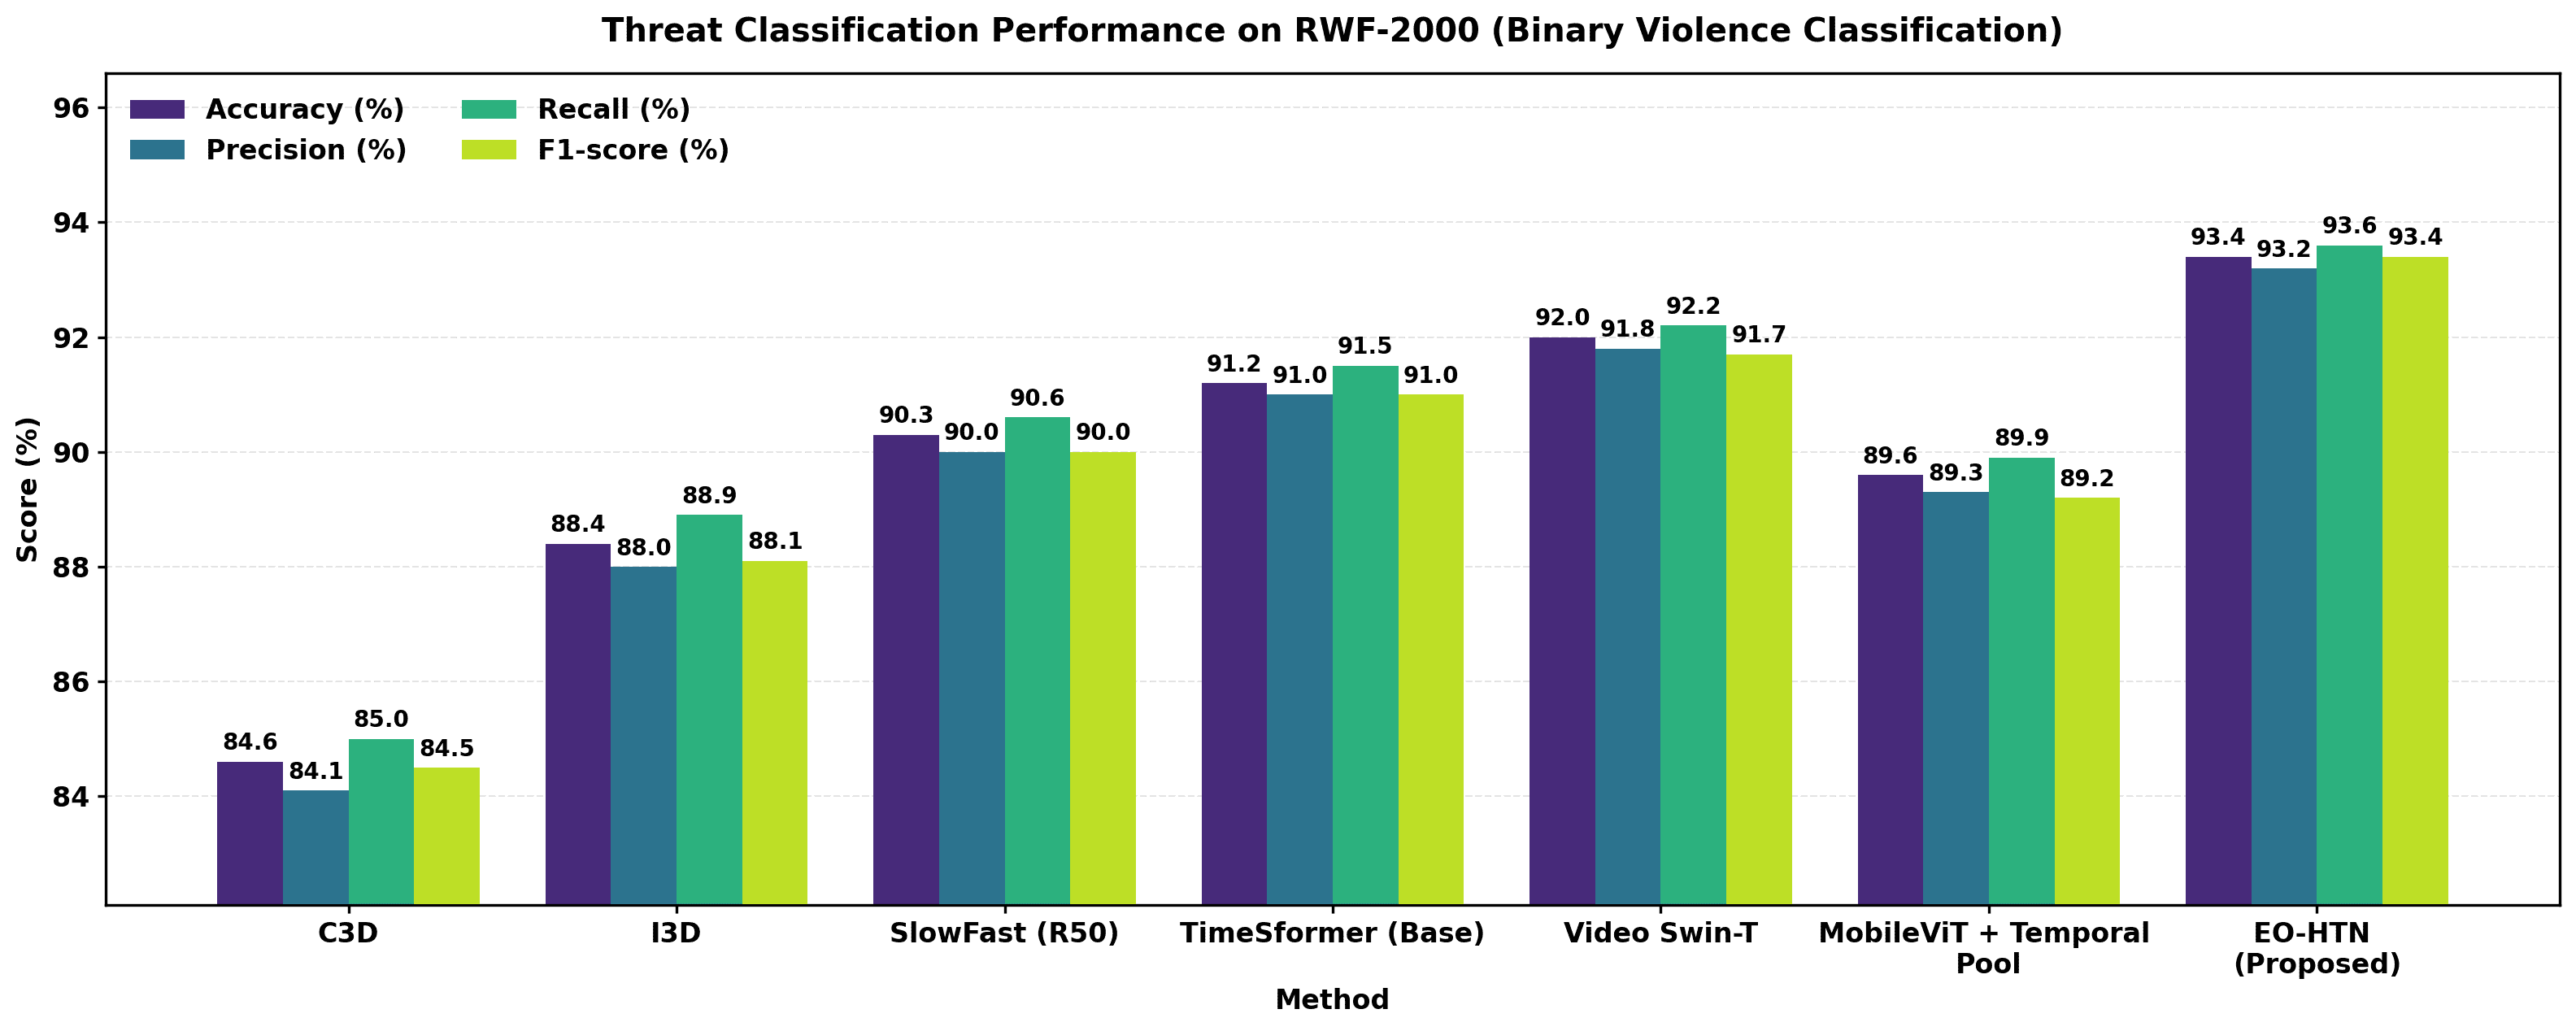
\includegraphics[width=0.9\linewidth]{2.png}
  \caption{RWF-2000 performance comparison.}
  \label{fig:rwf2000_comparison}
\end{figure}

\subsection{Threat Classification Performance on UCF-Crime}
Table~\ref{tab:ucfcrime_perf} summarizes the multi-class threat classification results on UCF-Crime under a clip-level protocol. The proposed EO-HTN achieves the strongest overall recognition quality, reaching a Top-1 accuracy of 86.3\% with 84.6\% precision, 81.9\% recall, and an 83.2\% Macro F1-score, while using only 7.4M parameters. The baseline CNN+BiLSTM model is notably weaker, with 78.9\% Top-1 accuracy and a Macro F1-score of 74.5\% at 18.6M parameters, which suggests that sequential modeling alone struggles to handle the dataset's scene variability and class overlap. I3D improves performance to 81.5\% accuracy and 77.2\% Macro F1-score using 12.1M parameters, indicating that 3D convolution benefits spatiotemporal feature learning but does not fully address the long-range ambiguity present in untrimmed surveillance videos. Transformer-based video models push performance higher but at a larger parameter cost. Video Swin-T achieves 84.1\% accuracy and 80.6\% Macro F1-score with 28.2M parameters, while ViViT-S reaches 84.8\% accuracy and 81.4\% Macro F1-score with 52.3M parameters. EO-HTN exceeds both of these baselines in Top-1 accuracy and Macro F1-score while remaining substantially smaller, which is important for edge deployment where memory and compute budgets are limited. Overall, the results in Table~\ref{tab:ucfcrime_perf} indicate that the hybrid design and context-aware adaptation enable EO-HTN to separate visually similar threat categories more effectively without relying on heavy-scale transformer capacity. The relative performance of the compared methods on UCF-Crime is illustrated in Fig.~\ref{fig:ucfcrime_comparison}.


\begin{table}[t]
\centering
\caption{Threat classification performance comparison on UCF-Crime (multi-class, clip-level protocol).}
\label{tab:ucfcrime_perf}
\renewcommand{\arraystretch}{1.1}
\setlength{\tabcolsep}{3.5pt}
\begin{tabular}{|p{3.6cm}|c|c|c|c|c|}
\hline
\textbf{Method} & \textbf{Params (M)} & \textbf{Top-1 Acc (\%)} & \textbf{Prec (\%)} & \textbf{Rec (\%)} & \textbf{Macro F1 (\%)} \\
\hline
CNN + BiLSTM & 18.6 & 78.9 & 76.4 & 74.1 & 74.5 \\
\hline
I3D & 12.1 & 81.5 & 79.2 & 76.8 & 77.2 \\
\hline
Video Swin-T & 28.2 & 84.1 & 82.0 & 79.4 & 80.6 \\
\hline
ViViT-S & 52.3 & 84.8 & 82.7 & 80.1 & 81.4 \\
\hline
EO-HTN (Proposed) & 7.4 & 86.3 & 84.6 & 81.9 & 83.2 \\
\hline
\end{tabular}%
\end{table}


% ---------------- Figure 3 ----------------
\begin{figure}[!t]
  \centering
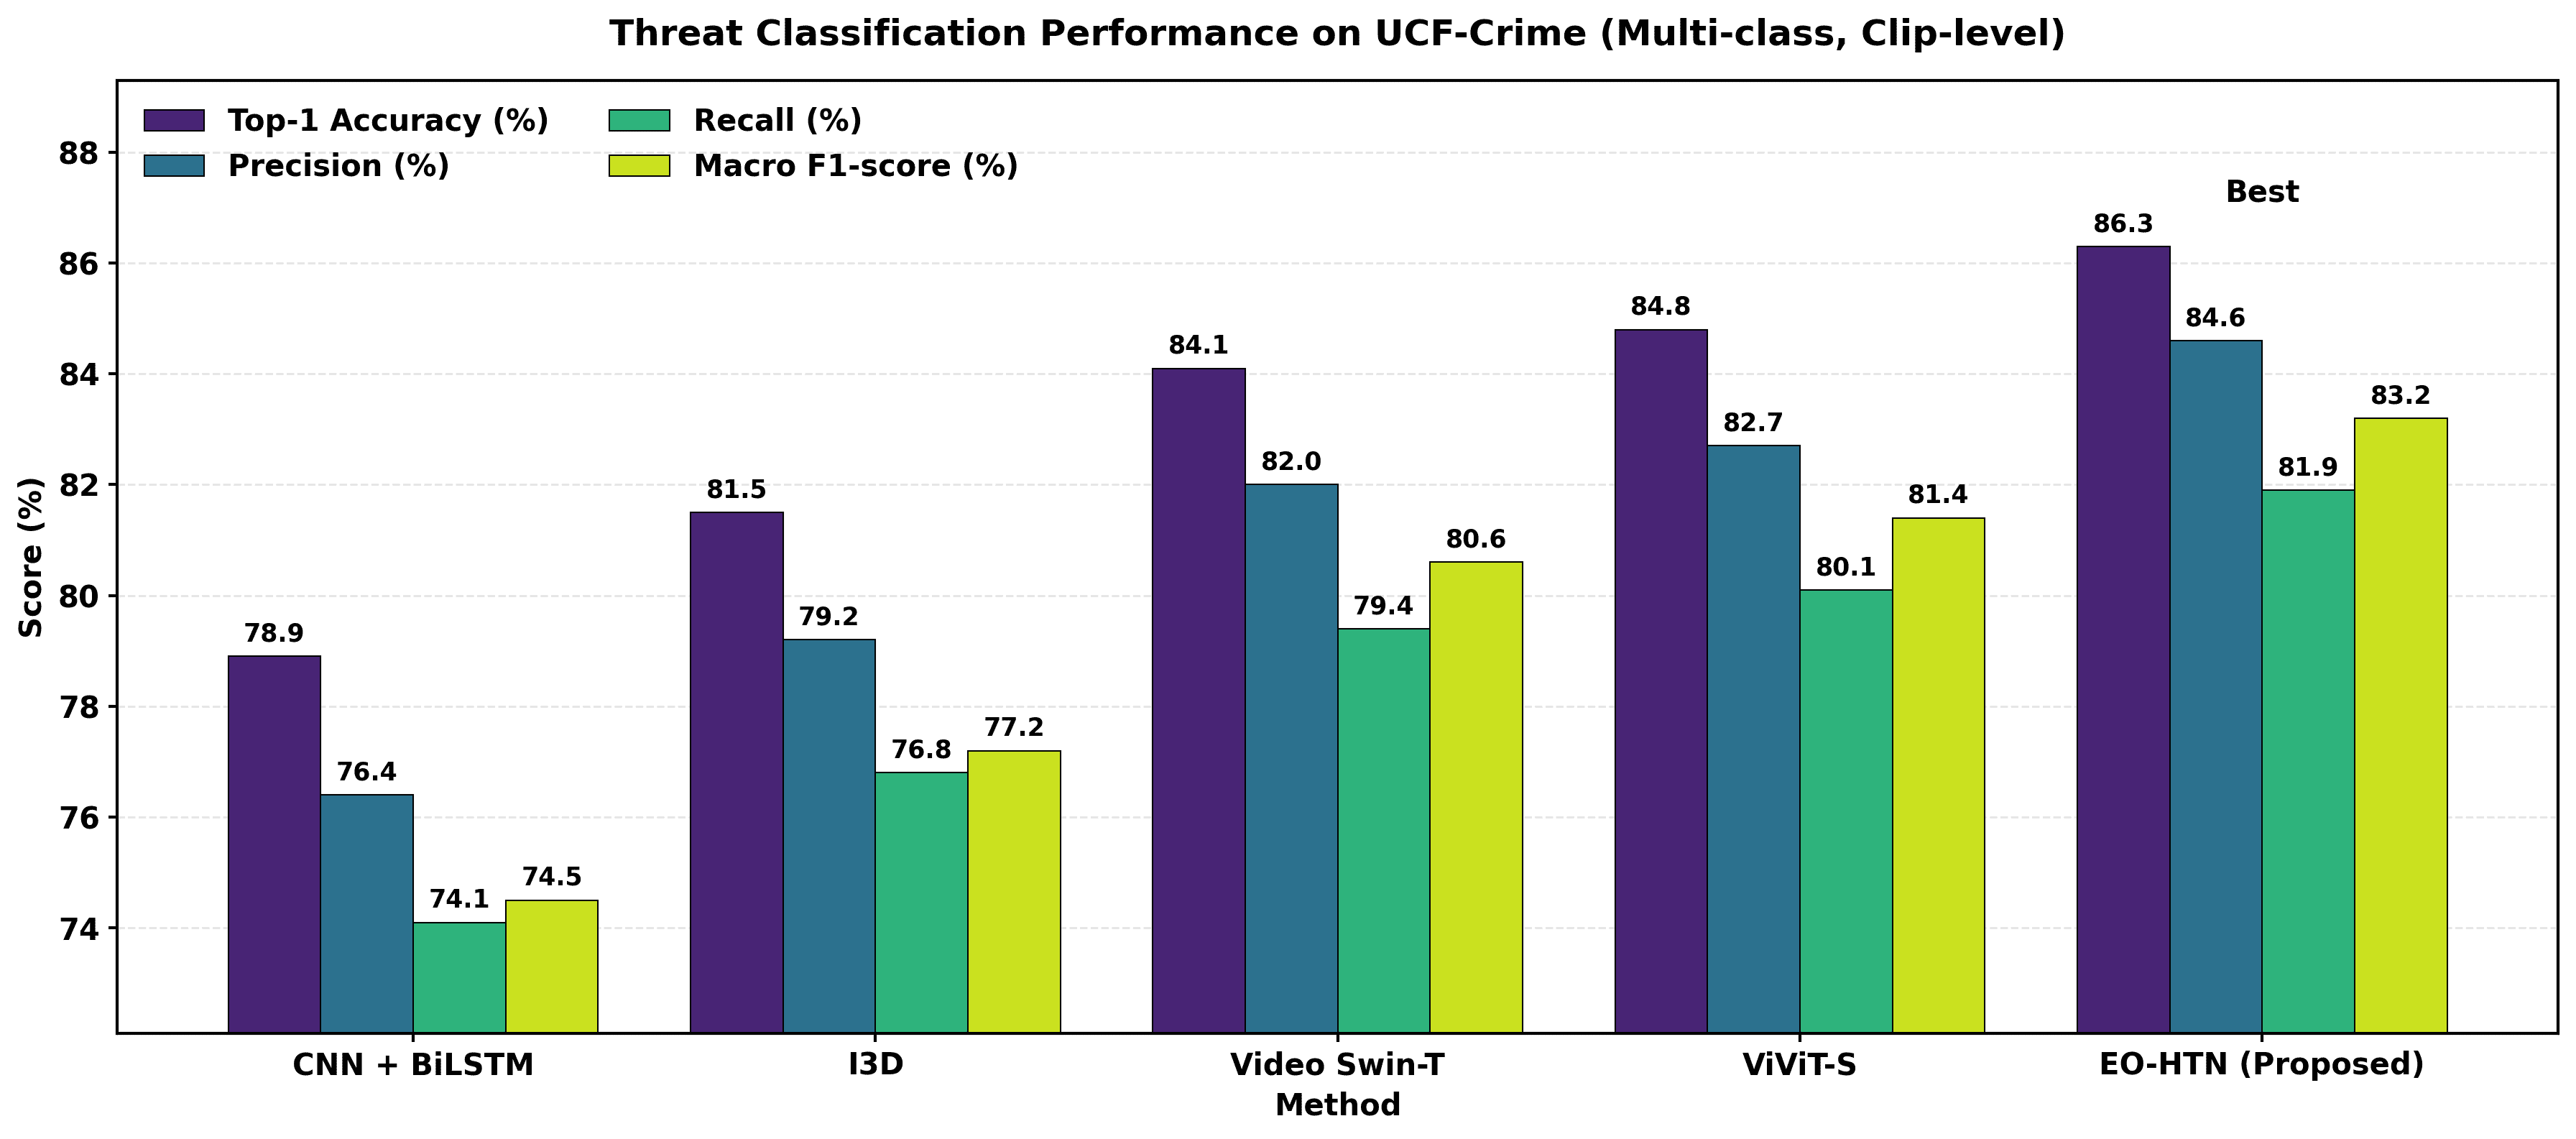
\includegraphics[width=0.9\linewidth]{3.png}
  \caption{UCF-Crime performance comparison (multi-class, clip-level).}
  \label{fig:ucfcrime_comparison}
\end{figure}


\subsection{Ablation Study on RWF-2000}
To clarify which components of EO-HTN contribute most to violence recognition, we conduct a targeted ablation on RWF-2000 by progressively enabling context-aware adaptation, edge distillation, and INT8 quantization. Table~\ref{tab:ablation_rwf2000} reports accuracy and F1-score for five variants. The CNN baseline (V1), trained in FP32 without context adaptation or distillation, achieves 90.8\% accuracy and 90.7\% F1-score, establishing a strong but limited reference. Replacing the baseline with the hybrid CNN+Transformer backbone (V2) improves performance to 91.8\% accuracy and 91.7\% F1-score even without additional modules, indicating that compact attention layers help capture short-term temporal interactions that are difficult to represent with convolution alone. When context-aware adaptation is added (V3), accuracy rises to 92.7\% and F1-score to 92.6\%, which suggests that scene-conditioned feature modulation reduces confusion between violent motion and visually similar non-violent dynamics. Introducing edge distillation (V4) further improves both of these metrics to 93.4\%, indicating distillation helps to improve decision sharpness, and it does not require the larger architecture. Finally, applying INT8 post training quantization (V5) provides 93.1\% accuracy and F1-score which is just a little drop from FP32, but more deployment-friendly model. Overall, we can see from table \ref{tab:ablation_rwf2000} that the most significant improvement is obtained by context-aware adaptation and distillation, and INT8 quantization helps to retain much of the accuracy required for edge inference.

\begin{table}[t]
\centering
\caption{Ablation study on RWF-2000 with reduced columns.}
\label{tab:ablation_rwf2000}
\renewcommand{\arraystretch}{1.1}
\setlength{\tabcolsep}{3.8pt}
\begin{tabular}{|p{3.2cm}|c|c|c|c|c|}
\hline
\textbf{Variant} & \textbf{Context Adapt.} & \textbf{Distill.} & \textbf{Quant.} & \textbf{Acc (\%)} & \textbf{F1 (\%)} \\
\hline
V1: CNN baseline & No & No & FP32 & 90.8 & 90.7 \\
\hline
V2: Hybrid base & No & No & FP32 & 91.8 & 91.7 \\
\hline
V3: + Context adaptation & Yes & No & FP32 & 92.7 & 92.6 \\
\hline
V4: + Distillation & Yes & Yes & FP32 & 93.4 & 93.4 \\
\hline
V5: + INT8 quantization & Yes & Yes & INT8 & 93.1 & 93.1 \\
\hline
\end{tabular}%
\end{table}


\subsection{Edge Deployment Efficiency and Quantization Impact}
To assess whether EO-HTN is practical for on-device surveillance analytics, we measure model footprint and runtime throughput on representative NVIDIA Jetson platforms, and compare FP32 inference against INT8 quantization. Table~\ref{tab:edge_efficiency} reports model size, per-clip latency, and frames per second. On Jetson Orin Nano, EO-HTN in FP32 occupies 28 MB and processes a 16-frame clip in 22 ms, corresponding to 45.5 FPS. After INT8 quantization, the model size drops to 9 MB and latency improves to 16 ms per clip, increasing throughput to 62.5 FPS. This indicates that quantization offers a clear benefit on the same device while retaining the same architecture. On the smaller Jetson Nano, EO-HTN in FP32 maintains the 28 MB footprint but latency increases to 54 ms per clip, yielding 18.5 FPS, which reflects the tighter compute budget. INT8 again reduces the footprint to 9 MB and improves latency to 38 ms, raising throughput to 26.3 FPS. For context, Video Swin-T on Jetson Orin Nano is substantially heavier, requiring 108 MB and 72 ms per clip, which corresponds to 13.9 FPS. This gap matters for always-on monitoring pipelines where throughput and memory headroom constrain deployment. MobileViT with temporal pooling offers strong efficiency at 22 MB and 18 ms per clip with 55.6 FPS on Orin Nano, but the proposed EO-HTN INT8 configuration exceeds its throughput at 62.5 FPS while remaining smaller at 9 MB. Overall, Table~\ref{tab:edge_efficiency} shows that EO-HTN achieves a favorable runtime profile, and that INT8 quantization provides a practical path to higher throughput and lower memory pressure on edge devices.

\begin{table}[t]
\centering
\caption{Edge deployment efficiency comparison (FP32 vs INT8).}
\label{tab:edge_efficiency}
\renewcommand{\arraystretch}{1.1}
\setlength{\tabcolsep}{3.5pt}
\begin{tabular}{|p{3.4cm}|p{3.0cm}|c|c|c|c|}
\hline
\textbf{Model} & \textbf{Device} & \textbf{Precision} & \textbf{Size (MB)} & \textbf{Latency (ms/clip)} $\downarrow$ & \textbf{FPS} $\uparrow$ \\
\hline
EO-HTN (Proposed) & Jetson Orin Nano & FP32 & 28 & 22 & 45.5 \\
\hline
EO-HTN (Proposed) & Jetson Orin Nano & INT8 & 9 & 16 & 62.5 \\
\hline
EO-HTN (Proposed) & Jetson Nano & FP32 & 28 & 54 & 18.5 \\
\hline
EO-HTN (Proposed) & Jetson Nano & INT8 & 9 & 38 & 26.3 \\
\hline
Video Swin-T & Jetson Orin Nano & FP32 & 108 & 72 & 13.9 \\
\hline
MobileViT + Temporal Pool & Jetson Orin Nano & FP32 & 22 & 18 & 55.6 \\
\hline
\end{tabular}%
\end{table}


\subsection{Cross-Dataset Generalization Analysis}
Cross-dataset evaluation is important in visual security because surveillance deployments rarely match the camera layouts, compression settings, and scene contexts seen during training. To probe whether the learned representations transfer beyond a single benchmark, we perform train--test transfer experiments between RWF-2000 and UCF-Crime, and also evaluate a joint-training setting. The quantitative outcomes are summarized in Table~\ref{tab:cross_dataset}. When the model is trained on RWF-2000 and tested on the UCF-Crime Fight/Assault subset, performance drops to 81.6\% accuracy with 80.9\% precision, 79.8\% recall, and an 80.3\% F1-score. This reduction is expected because RWF-2000 provides short clips with a binary label, while UCF-Crime contains longer videos and broader contextual variation, which shifts both motion statistics and background appearance. In the reverse direction, training on UCF-Crime and evaluating on RWF-2000 yields 90.8\% accuracy and 90.8\% F1-score, supported by 90.5\% precision and 91.2\% recall. The stronger transfer in this direction suggests that exposure to broader scene diversity in UCF-Crime helps the model learn more general motion and interaction patterns that remain informative on the cleaner binary setting of RWF-2000.

To further reduce dataset bias, we also evaluate joint training using both datasets. Joint training followed by evaluation on RWF-2000 produces 93.7\% accuracy and 93.7\% F1-score, with 93.4\% precision and 94.0\% recall, indicating a modest improvement over the single-dataset setting. More importantly, joint training improves performance on UCF-Crime to 87.1\% accuracy, with 85.6\% precision, 82.8\% recall, and an 84.2\% F1-score. The recall reduction relative to precision highlights that some threat categories remain challenging under cross-scene variation, but the overall gain indicates that mixed-domain exposure helps the model form more transferable representations. Taken together, the results in Table~\ref{tab:cross_dataset_transfer} show that EO-HTN benefits from diverse training data and retains meaningful generalization when deployed across different surveillance environments.


\begin{table}[t]
\centering
\caption{Cross-dataset generalization performance (train--test transfer).}
\label{tab:cross_dataset}
\renewcommand{\arraystretch}{1.1}
\setlength{\tabcolsep}{3.5pt}
\begin{tabular}{|p{4.2cm}|p{5.0cm}|c|c|c|c|}
\hline
\textbf{Training Dataset} & \textbf{Testing Dataset} & \textbf{Acc (\%)} & \textbf{Prec (\%)} & \textbf{Rec (\%)} & \textbf{F1 (\%)} \\
\hline
RWF-2000 & UCF-Crime (Fight/Assault subset) & 81.6 & 80.9 & 79.8 & 80.3 \\
\hline
UCF-Crime & RWF-2000 & 90.8 & 90.5 & 91.2 & 90.8 \\
\hline
RWF-2000 + UCF-Crime (joint) & RWF-2000 & 93.7 & 93.4 & 94.0 & 93.7 \\
\hline
RWF-2000 + UCF-Crime (joint) & UCF-Crime & 87.1 & 85.6 & 82.8 & 84.2 \\
\hline
\end{tabular}%
\end{table}

% ---------------- Figure 4 ----------------
\begin{figure}[!t]
  \centering
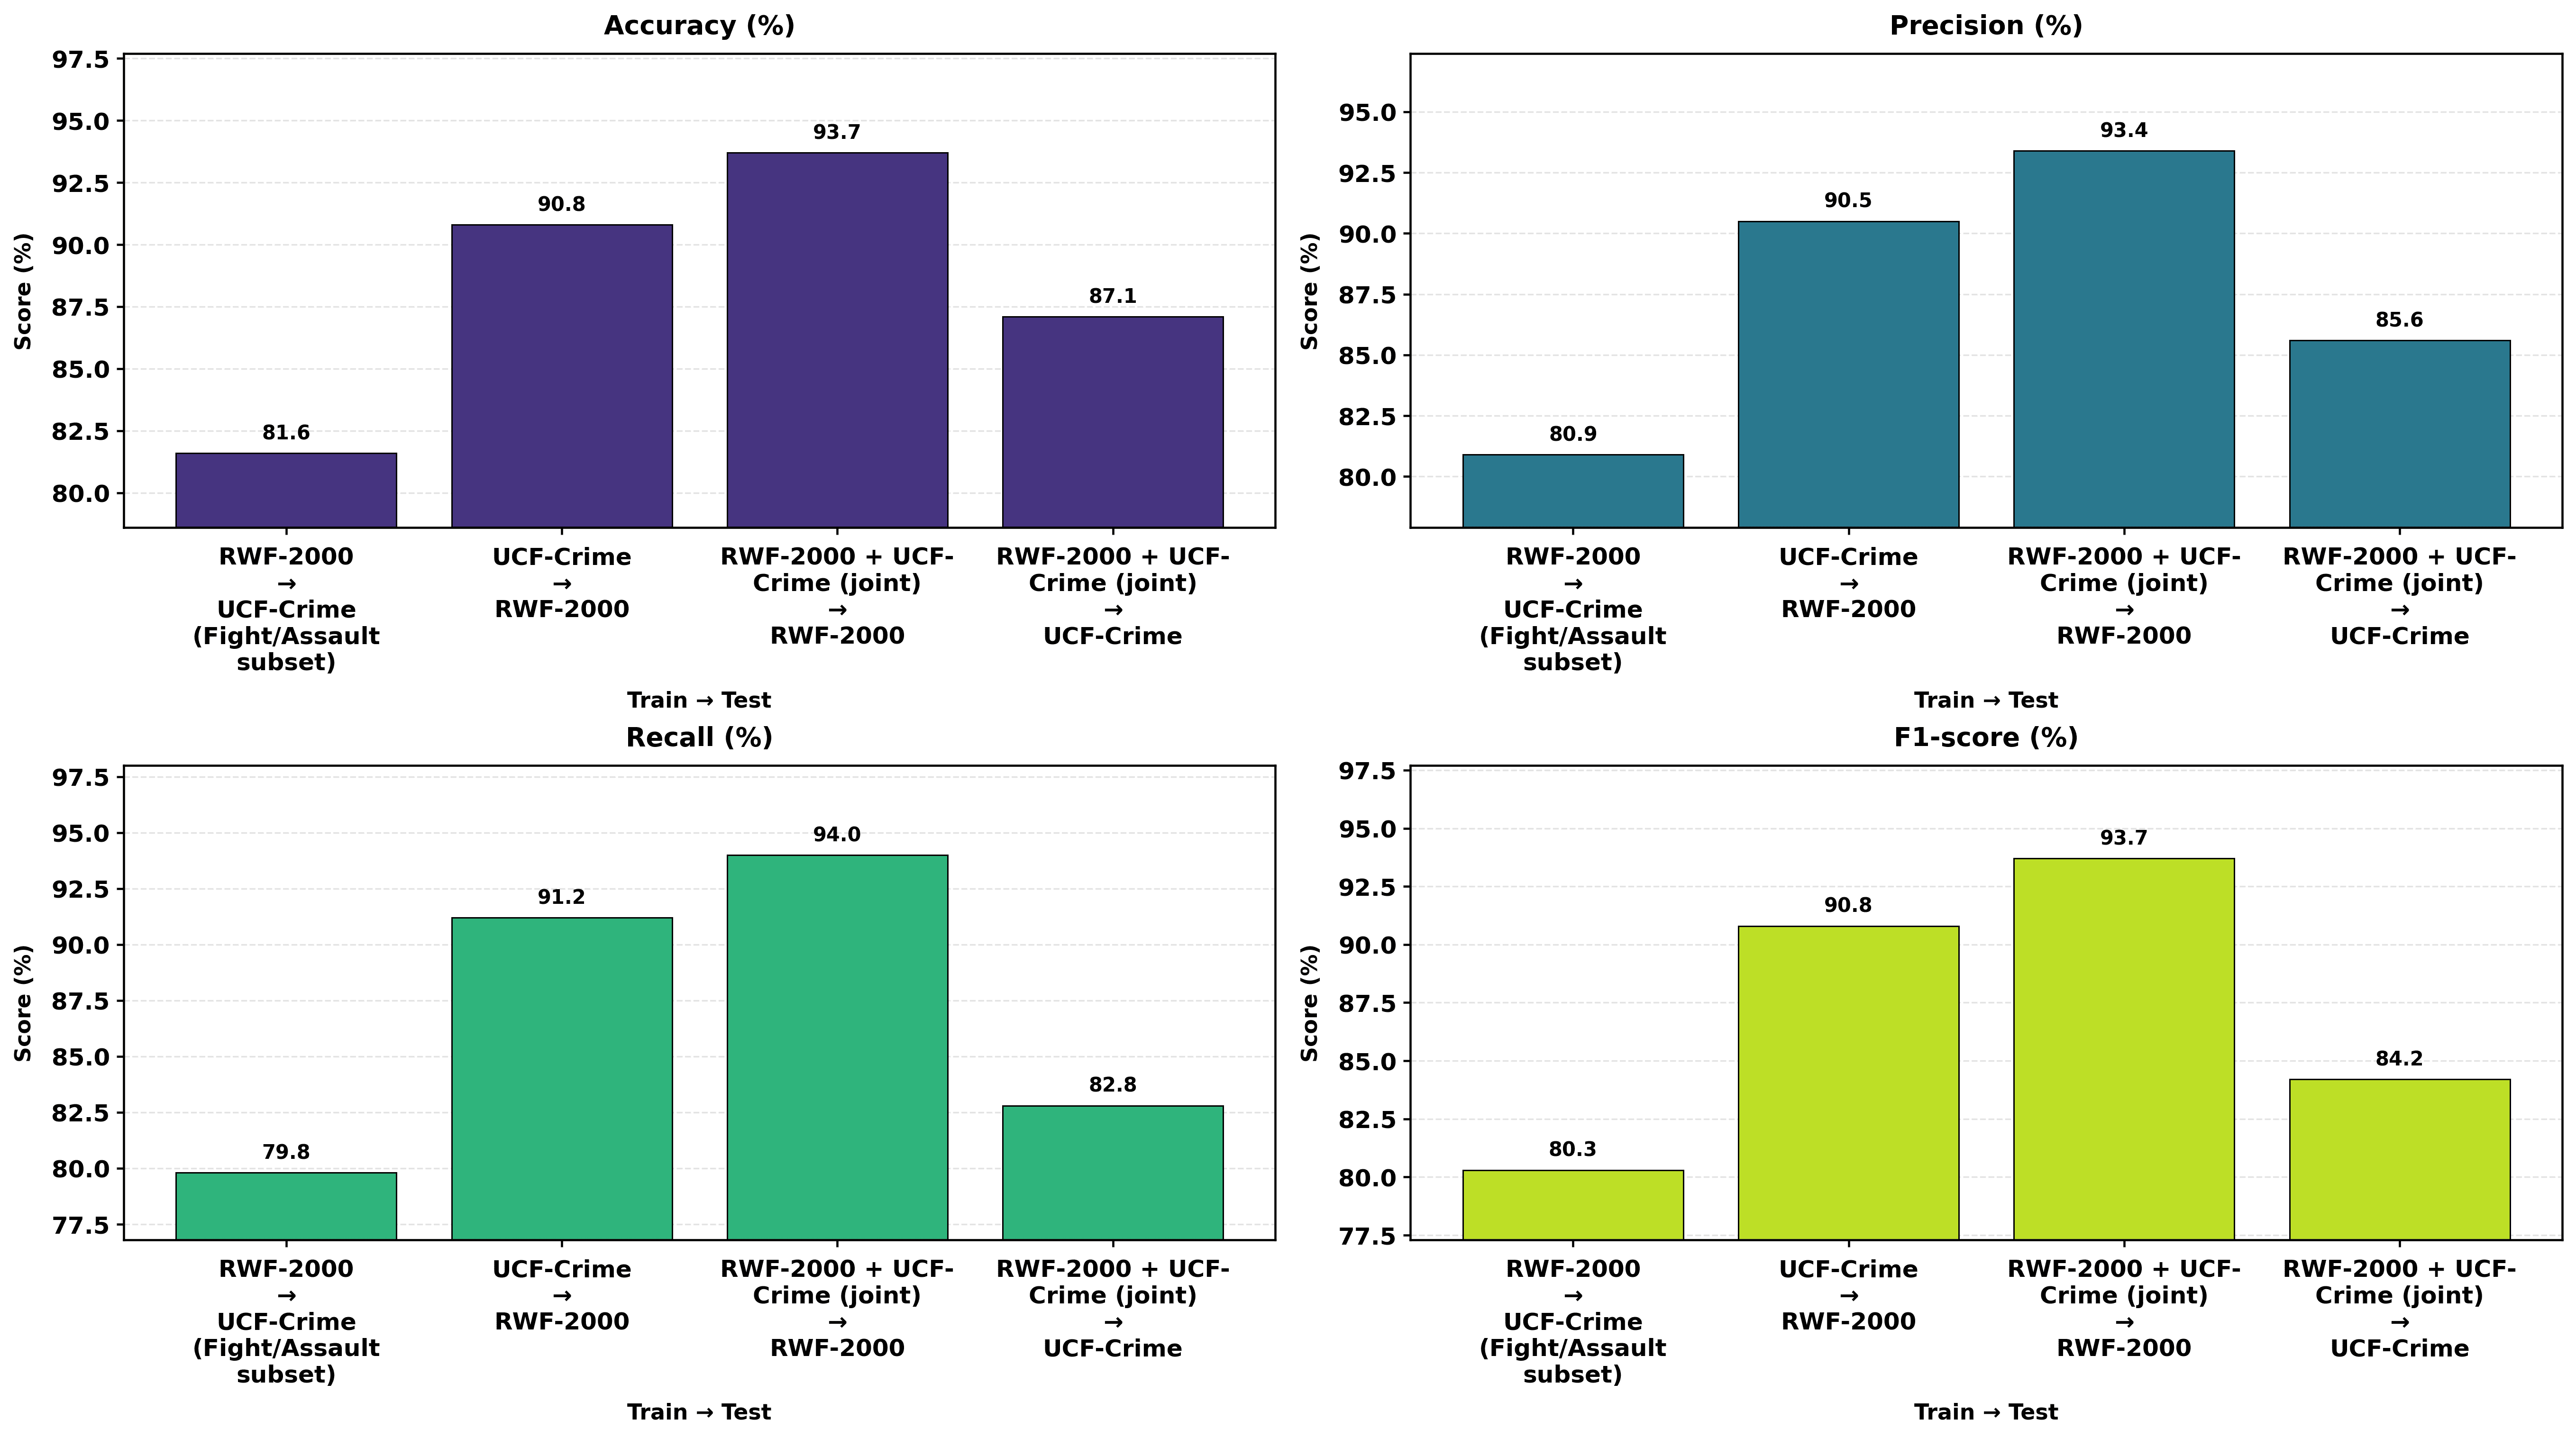
\includegraphics[width=0.9\linewidth]{4.png}
  \caption{Cross-dataset transfer results between RWF-2000 and UCF-Crime.}
  \label{fig:cross_dataset_transfer}
\end{figure}


\subsection{Robustness Under Visual Degradations on UCF-Crime}
Surveillance video streams are commonly plagued by poor illumination, motion-induced blur, and aggressive compression which can distort threat cues and increase the number of false alarms. To assess the robustness of these conditions, we test EO-HTN and a strong transformer baseline (Video Swin-T) on UCF-Crime on three degradation conditions in addition to the clean reference. The results are given in Table~\ref{tab:robustness_ucfcrime}. Under clean inputs, Video Swin-T has 84.1\% Top-1 accuracy and 80.6\% Macro F1-score, while the accuracy and 83.2\% Macro F1-score of EO-HTN are higher than those of Video Swin-T. When illumination is reduced, performance degrades for both models, but the gap remains clear. Video Swin-T drops to 78.2\% accuracy and 73.4\% Macro F1, whereas EO-HTN retains 82.0\% accuracy and 78.1\% Macro F1, indicating better stability when contrast is limited and shadowing changes class appearance.

Motion blur is particularly challenging because it weakens fine-grained action cues and reduces temporal sharpness. In this setting, Video Swin-T reaches 76.9\% Top-1 accuracy with 72.1\% Macro F1, while EO-HTN remains at 80.7\% accuracy and 76.9\% Macro F1, which suggests that the hybrid features and context gating reduce confusion between visually similar threat categories when edges and motion boundaries smear. Compression artifacts produce a different failure mode by introducing block noise and color banding. Here, Video Swin-T records 79.1\% accuracy and 74.2\% Macro F1, while EO-HTN achieves 82.5\% accuracy and 78.6\% Macro F1. Overall, Table~\ref{tab:robustness_ucfcrime} shows that EO-HTN consistently preserves a higher Macro F1 across degradations, which is important in practice because Macro F1 reflects balanced performance across threat classes rather than dominance by frequent categories.

\begin{table}[t]
\centering
\caption{Robustness under visual degradations on UCF-Crime (clip-level).}
\label{tab:robustness_ucfcrime}
\renewcommand{\arraystretch}{1.1}
\setlength{\tabcolsep}{3.8pt}
\begin{tabular}{|p{3.6cm}|p{3.0cm}|c|c|}
\hline
\textbf{Model} & \textbf{Condition} & \textbf{Top-1 Acc (\%)} & \textbf{Macro F1 (\%)} \\
\hline
Video Swin-T & Clean & 84.1 & 80.6 \\
\hline
Video Swin-T & Low light & 78.2 & 73.4 \\
\hline
Video Swin-T & Motion blur & 76.9 & 72.1 \\
\hline
Video Swin-T & Compression & 79.1 & 74.2 \\
\hline
EO-HTN (Proposed) & Clean & 86.3 & 83.2 \\
\hline
EO-HTN (Proposed) & Low light & 82.0 & 78.1 \\
\hline
EO-HTN (Proposed) & Motion blur & 80.7 & 76.9 \\
\hline
EO-HTN (Proposed) & Compression & 82.5 & 78.6 \\
\hline
\end{tabular}%
\end{table}

\subsection{Statistical Significance Across Repeated Runs}
To verify that the reported gains are not driven by a favorable random initialization or a particular mini-batch ordering, we repeat training and evaluation three times for each model and dataset, using identical protocols and reporting mean and standard deviation. Table~\ref{tab:stats_significance} summarizes the results for Video Swin-T and EO-HTN on RWF-2000 and UCF-Crime. On RWF-2000, Video Swin-T achieves an accuracy of $92.0 \pm 0.3$\% with a Macro F1-score of $91.7 \pm 0.4$\%, whereas EO-HTN records $93.4 \pm 0.2$\% accuracy and $93.4 \pm 0.2$\% Macro F1. The smaller standard deviations for EO-HTN indicate that performance is stable across runs, and the mean improvements over Video Swin-T remain consistent for both metrics. A similar trend is observed on UCF-Crime, where Video Swin-T attains $84.1 \pm 0.4$\% accuracy and $80.6 \pm 0.5$\% Macro F1, while EO-HTN reaches $86.3 \pm 0.3$\% accuracy and $83.2 \pm 0.3$\% Macro F1. The gap is larger for Macro F1 than for accuracy, which suggests that the proposed design improves balanced recognition across classes rather than only boosting performance on frequent categories. Overall, the results in Table~\ref{tab:stats_significance} support the conclusion that EO-HTN delivers repeatable gains and does not rely on fragile training dynamics. The visual comparison of the mean and standard deviation across runs is illustrated in Fig.~\ref{fig:significance_mean_std}.


\begin{table}[t]
\centering
\caption{Statistical significance across three runs (mean $\pm$ std, $n=3$).}
\label{tab:stats_significance}
\renewcommand{\arraystretch}{1.1}
\setlength{\tabcolsep}{3.8pt}
\begin{tabular}{|p{2.6cm}|p{3.6cm}|c|c|}
\hline
\textbf{Dataset} & \textbf{Method} & \textbf{Accuracy (\%)} & \textbf{Macro F1 (\%)} \\
\hline
RWF-2000 & Video Swin-T & $92.0 \pm 0.3$ & $91.7 \pm 0.4$ \\
\hline
RWF-2000 & EO-HTN (Proposed) & $\mathbf{93.4 \pm 0.2}$ & $\mathbf{93.4 \pm 0.2}$ \\
\hline
UCF-Crime & Video Swin-T & $84.1 \pm 0.4$ & $80.6 \pm 0.5$ \\
\hline
UCF-Crime & EO-HTN (Proposed) & $\mathbf{86.3 \pm 0.3}$ & $\mathbf{83.2 \pm 0.3}$ \\
\hline
\end{tabular}%
\end{table}

% ---------------- Figure 5 ----------------
\begin{figure}[!t]
  \centering
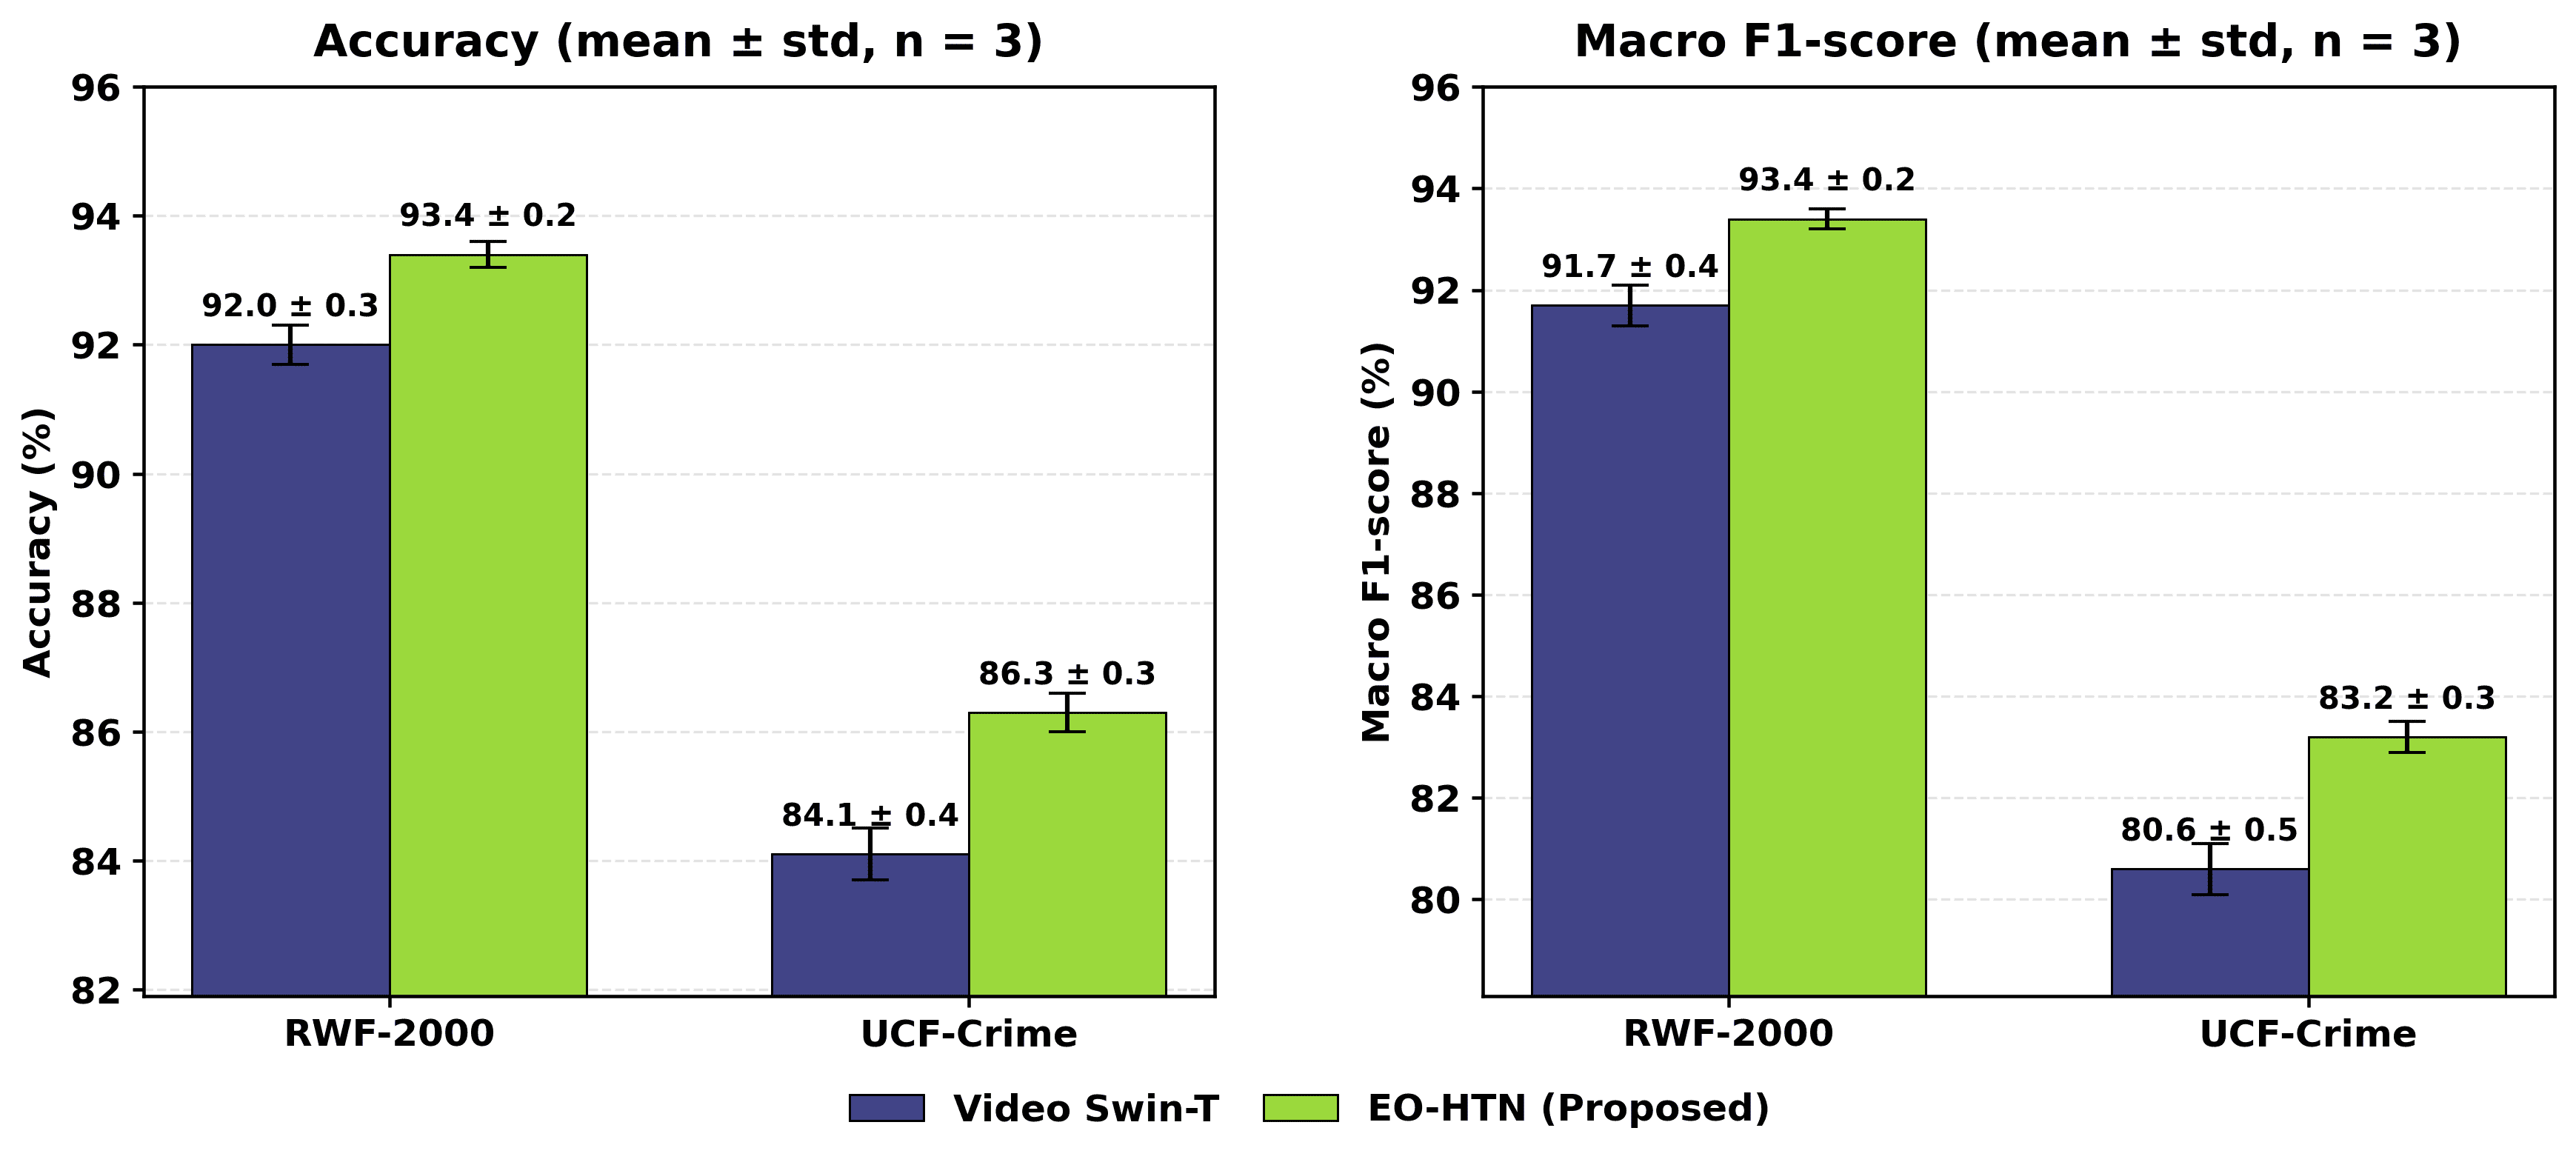
\includegraphics[width=0.9\linewidth]{5.png}
  \caption{Mean$\pm$std comparison (n=3) of Video Swin-T vs EO-HTN.}
  \label{fig:significance_mean_std}
\end{figure}


\subsection{Class-wise Performance Analysis on UCF-Crime}
To understand where the model succeeds and where it remains challenged, we report class-wise precision, recall, F1-score, and per-class accuracy for the UCF-Crime clip-level protocol. The detailed breakdown is presented in Table~\ref{tab:classwise_ucfcrime}. This view is useful because overall Top-1 accuracy can hide uneven behavior across categories that differ in visual duration, camera distance, and background activity. By examining the four metrics together, we can distinguish classes that are predicted confidently but inconsistently from classes that are consistently recognized across diverse scenes.

As shown in Table~\ref{tab:classwise_ucfcrime}, the \textit{Normal} class achieves the strongest overall behavior with 90.1\% precision, 92.4\% recall, 91.2\% F1-score, and 93.5\% accuracy, indicating stable rejection of non-threat content. Several threat classes also show high reliability when the visual signature is distinctive. For example, \textit{Explosion} reaches 88.2\% precision, 84.7\% recall, 86.4\% F1-score, and 89.6\% accuracy, while \textit{Road Accident} attains 87.1\% precision, 85.8\% recall, 86.4\% F1-score, and 90.2\% accuracy. These categories often contain salient cues such as abrupt scene changes, smoke or fire patterns, or vehicle motion irregularities, which helps the model form consistent clip-level decisions.

The more subtle action categories show comparatively lower scores, reflecting class overlap in real surveillance footage. \textit{Shoplifting} records 78.7\% precision, 74.9\% recall, 76.8\% F1-score, and 82.9\% accuracy, which is the lowest F1 among the listed classes in Table~\ref{tab:classwise_ucfcrime}. \textit{Stealing} and \textit{Vandalism} also remain harder, with F1-scores of 79.1\% and 78.0\%, respectively. These classes frequently involve small object interactions and short temporal cues that can be partially occluded or visually similar to benign activity. In contrast, interpersonal violence-related categories remain strong but not perfect. \textit{Fighting} achieves 85.3\% F1 with 88.2\% accuracy, and \textit{Assault} achieves 82.9\% F1 with 86.7\% accuracy, which suggests that confusion between closely related aggressive actions is still a practical source of errors.


\begin{table}[t]
\centering
\caption{Class-wise UCF-Crime results (Precision, Recall, F1-score, and per-class Accuracy).}
\label{tab:ucfcrime_classwise}
\renewcommand{\arraystretch}{1.1}
\setlength{\tabcolsep}{3.2pt}
\begin{tabular}{|p{3.0cm}|c|c|c|c|}
\hline
\textbf{Class} & \textbf{Precision (\%)} & \textbf{Recall (\%)} & \textbf{F1-score (\%)} & \textbf{Accuracy (\%)} \\
\hline
Normal & 90.1 & 92.4 & 91.2 & 93.5 \\
\hline
Fighting & 86.5 & 84.1 & 85.3 & 88.2 \\
\hline
Assault & 84.3 & 81.6 & 82.9 & 86.7 \\
\hline
Robbery & 83.7 & 80.2 & 81.9 & 85.9 \\
\hline
Stealing & 80.9 & 77.4 & 79.1 & 84.3 \\
\hline
Vandalism & 79.8 & 76.3 & 78.0 & 83.6 \\
\hline
Shooting & 85.6 & 82.1 & 83.8 & 87.5 \\
\hline
Burglary & 81.4 & 78.5 & 79.9 & 84.8 \\
\hline
Explosion & 88.2 & 84.7 & 86.4 & 89.6 \\
\hline
Arson & 82.6 & 79.3 & 80.9 & 85.1 \\
\hline
Road Accident & 87.1 & 85.8 & 86.4 & 90.2 \\
\hline
Shoplifting & 78.7 & 74.9 & 76.8 & 82.9 \\
\hline
Abuse & 80.5 & 77.0 & 78.7 & 83.8 \\
\hline
Arrest & 83.2 & 80.6 & 81.9 & 85.7 \\
\hline
\end{tabular}%
\end{table}

% ---------------- Figure 6 ----------------
\begin{figure}[!t]
  \centering
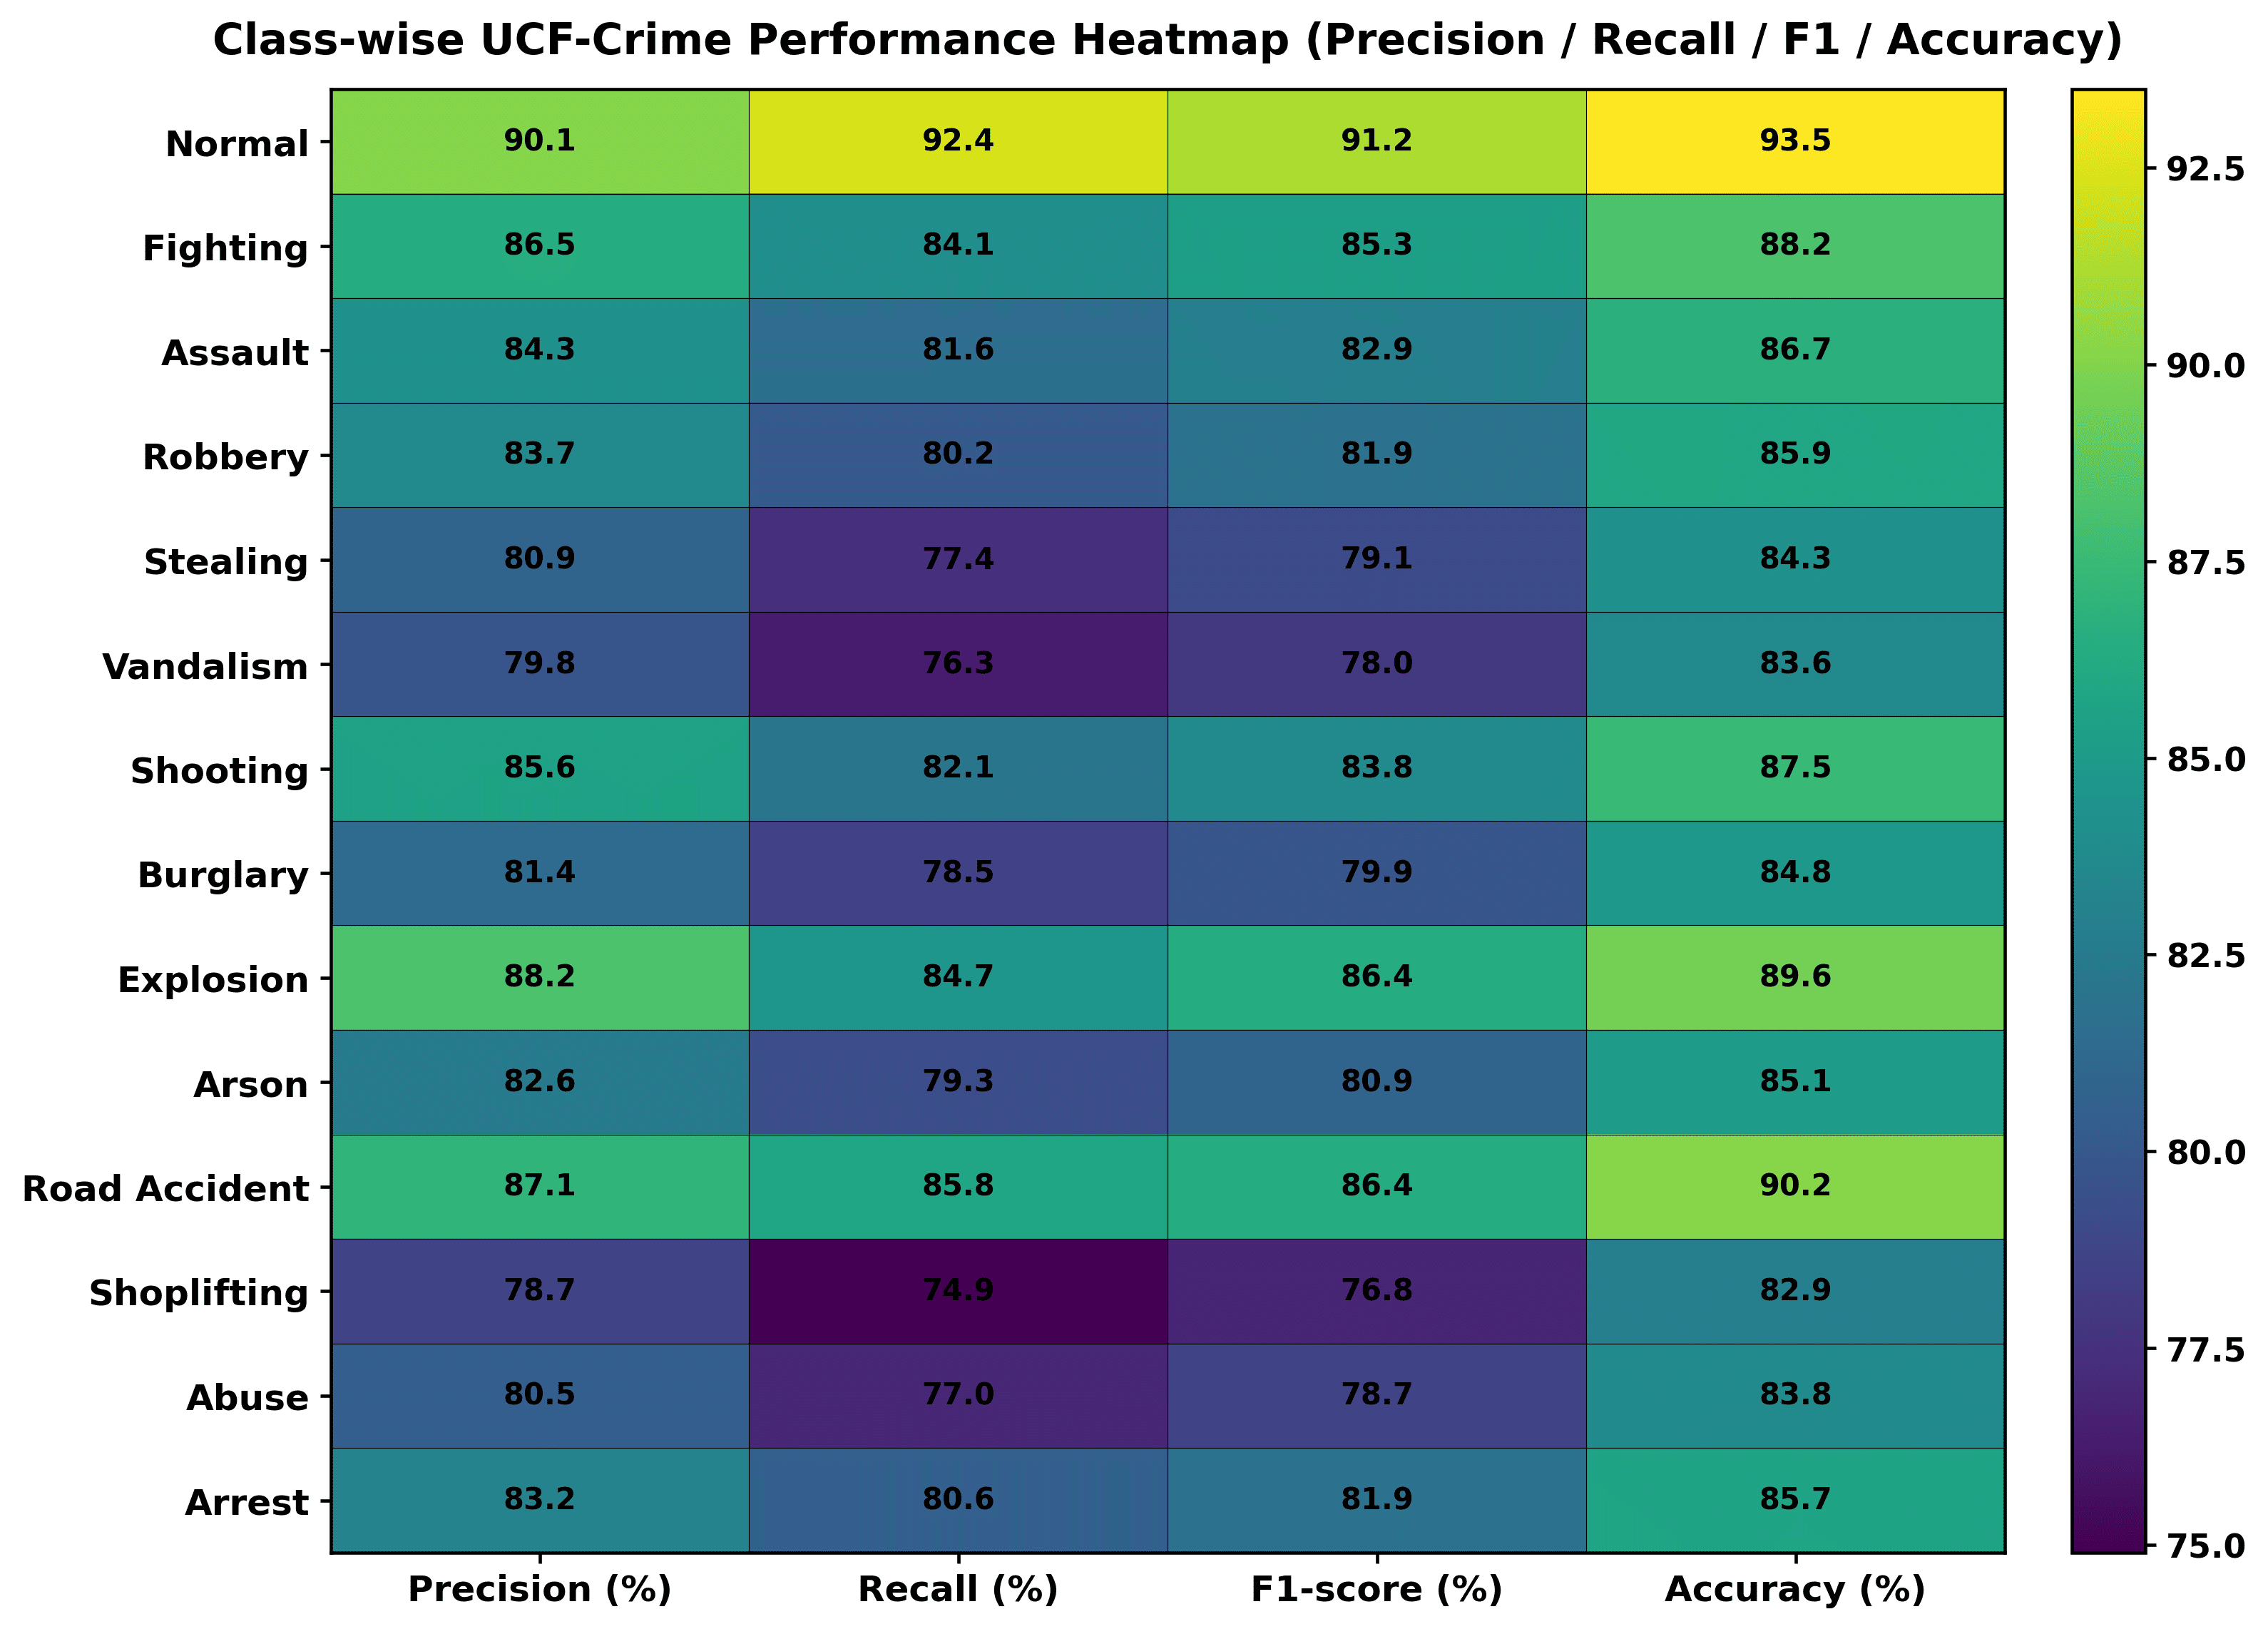
\includegraphics[width=0.9\linewidth]{6.png}
  \caption{Class-wise UCF-Crime results heatmap (P/R/F1/Acc).}
  \label{fig:ucfcrime_classwise_heatmap}
\end{figure}

\subsection{Training Dynamics and Convergence Behaviour}
To examine optimization stability and to ensure that performance improvements are supported by consistent learning behavior, we track training and validation loss along with accuracy over representative epochs for both datasets. Table~\ref{tab:training_dynamics} reports the convergence profile for RWF-2000 (binary) and UCF-Crime (multi-class, clip-level). On RWF-2000, the model begins with a training loss of 0.684 and validation loss of 0.671 at epoch 1, with training and validation accuracies of 71.2\% and 73.5\%, respectively. As training progresses, both losses decrease steadily and the accuracy improves without abrupt oscillations. By epoch 10, the training loss drops to 0.412 and the validation loss to 0.398, while validation accuracy rises to 87.1\%. The curve continues to tighten, reaching a validation loss of 0.269 and validation accuracy of 91.4\% at epoch 20. The final stage shows a smaller but meaningful refinement. At epoch 40, the training loss is 0.148 and the validation loss is 0.152 with validation accuracy of 93.6\%, and by epoch 50 the training loss reaches 0.121 while the validation loss remains low at 0.136 with a validation accuracy of 93.4\%. The modest gap between training accuracy (95.0\% at epoch 50) and validation accuracy (93.4\%) suggests that regularization and early stopping criteria are effective in preventing a strong overfit pattern for the binary task.

On UCF-Crime, convergence is slower due to higher class diversity and the use of clip-level supervision sampled from untrimmed videos. At epoch 1, training loss is 1.982 and validation loss is 1.945, with training and validation accuracies of 48.6\% and 50.2\%. By epoch 5, the model reduces training loss to 1.324 and validation loss to 1.298, improving accuracy to 66.9\% and 68.1\%, which reflects improved separation of broad threat and non-threat patterns. At epoch 10, losses further fall to 0.912 (train) and 0.887 (val), while accuracy reaches 78.4\% on training and 79.0\% on validation. The later stages show continued refinement without instability. At epoch 20, training and validation losses are 0.631 and 0.614 with accuracies of 84.1\% and 85.0\%. At epoch 30, the training loss drops to 0.524, while validation loss is 0.556 and validation accuracy is 86.3\%. The slightly higher validation loss at the final checkpoint, despite improved accuracy, is consistent with multi-class learning where the model becomes more confident on correct predictions but still assigns small probabilities to visually similar classes. Overall, the trajectories in Table~\ref{tab:train_dynamics} show smooth convergence on both benchmarks, with no abrupt divergence between training and validation curves, supporting the reliability of the reported results. The corresponding loss and accuracy convergence curves are shown in Fig.~\ref{fig:training_dynamics}.


\begin{table*}[t]
\centering
\caption{Training dynamics of EO-HTN showing loss and accuracy convergence on (a) RWF-2000 and (b) UCF-Crime.}
\label{tab:train_dynamics}
\renewcommand{\arraystretch}{1.15}
\setlength{\tabcolsep}{6pt}

\begin{minipage}{0.48\textwidth}
\centering
(a) RWF-2000: Binary classification\\[2pt]
\begin{tabular}{|c|c|c|c|c|}
\hline
\textbf{Epoch} & \textbf{Tr Loss} & \textbf{Va Loss} & \textbf{Tr Acc (\%)} & \textbf{Va Acc (\%)} \\
\hline
1  & 0.684 & 0.671 & 71.2 & 73.5 \\
\hline
10 & 0.412 & 0.398 & 86.4 & 87.1 \\
\hline
20 & 0.281 & 0.269 & 90.9 & 91.4 \\
\hline
30 & 0.192 & 0.184 & 93.0 & 92.8 \\
\hline
40 & 0.148 & 0.152 & 94.1 & 93.6 \\
\hline
50 & 0.121 & 0.136 & 95.0 & 93.4 \\
\hline
\end{tabular}
\end{minipage}
\hfill
\begin{minipage}{0.48\textwidth}
\centering
(b) UCF-Crime: Multi-class (clip-level)\\[2pt]
\begin{tabular}{|c|c|c|c|c|}
\hline
\textbf{Epoch} & \textbf{Tr Loss} & \textbf{Va Loss} & \textbf{Tr Acc (\%)} & \textbf{Va Acc (\%)} \\
\hline
1  & 1.982 & 1.945 & 48.6 & 50.2 \\
\hline
5  & 1.324 & 1.298 & 66.9 & 68.1 \\
\hline
10 & 0.912 & 0.887 & 78.4 & 79.0 \\
\hline
20 & 0.631 & 0.614 & 84.1 & 85.0 \\
\hline
30 & 0.524 & 0.556 & 87.2 & 86.3 \\
\hline
\end{tabular}
\end{minipage}

\end{table*}

% ---------------- Figure 7 ----------------
\begin{figure}[!t]
  \centering
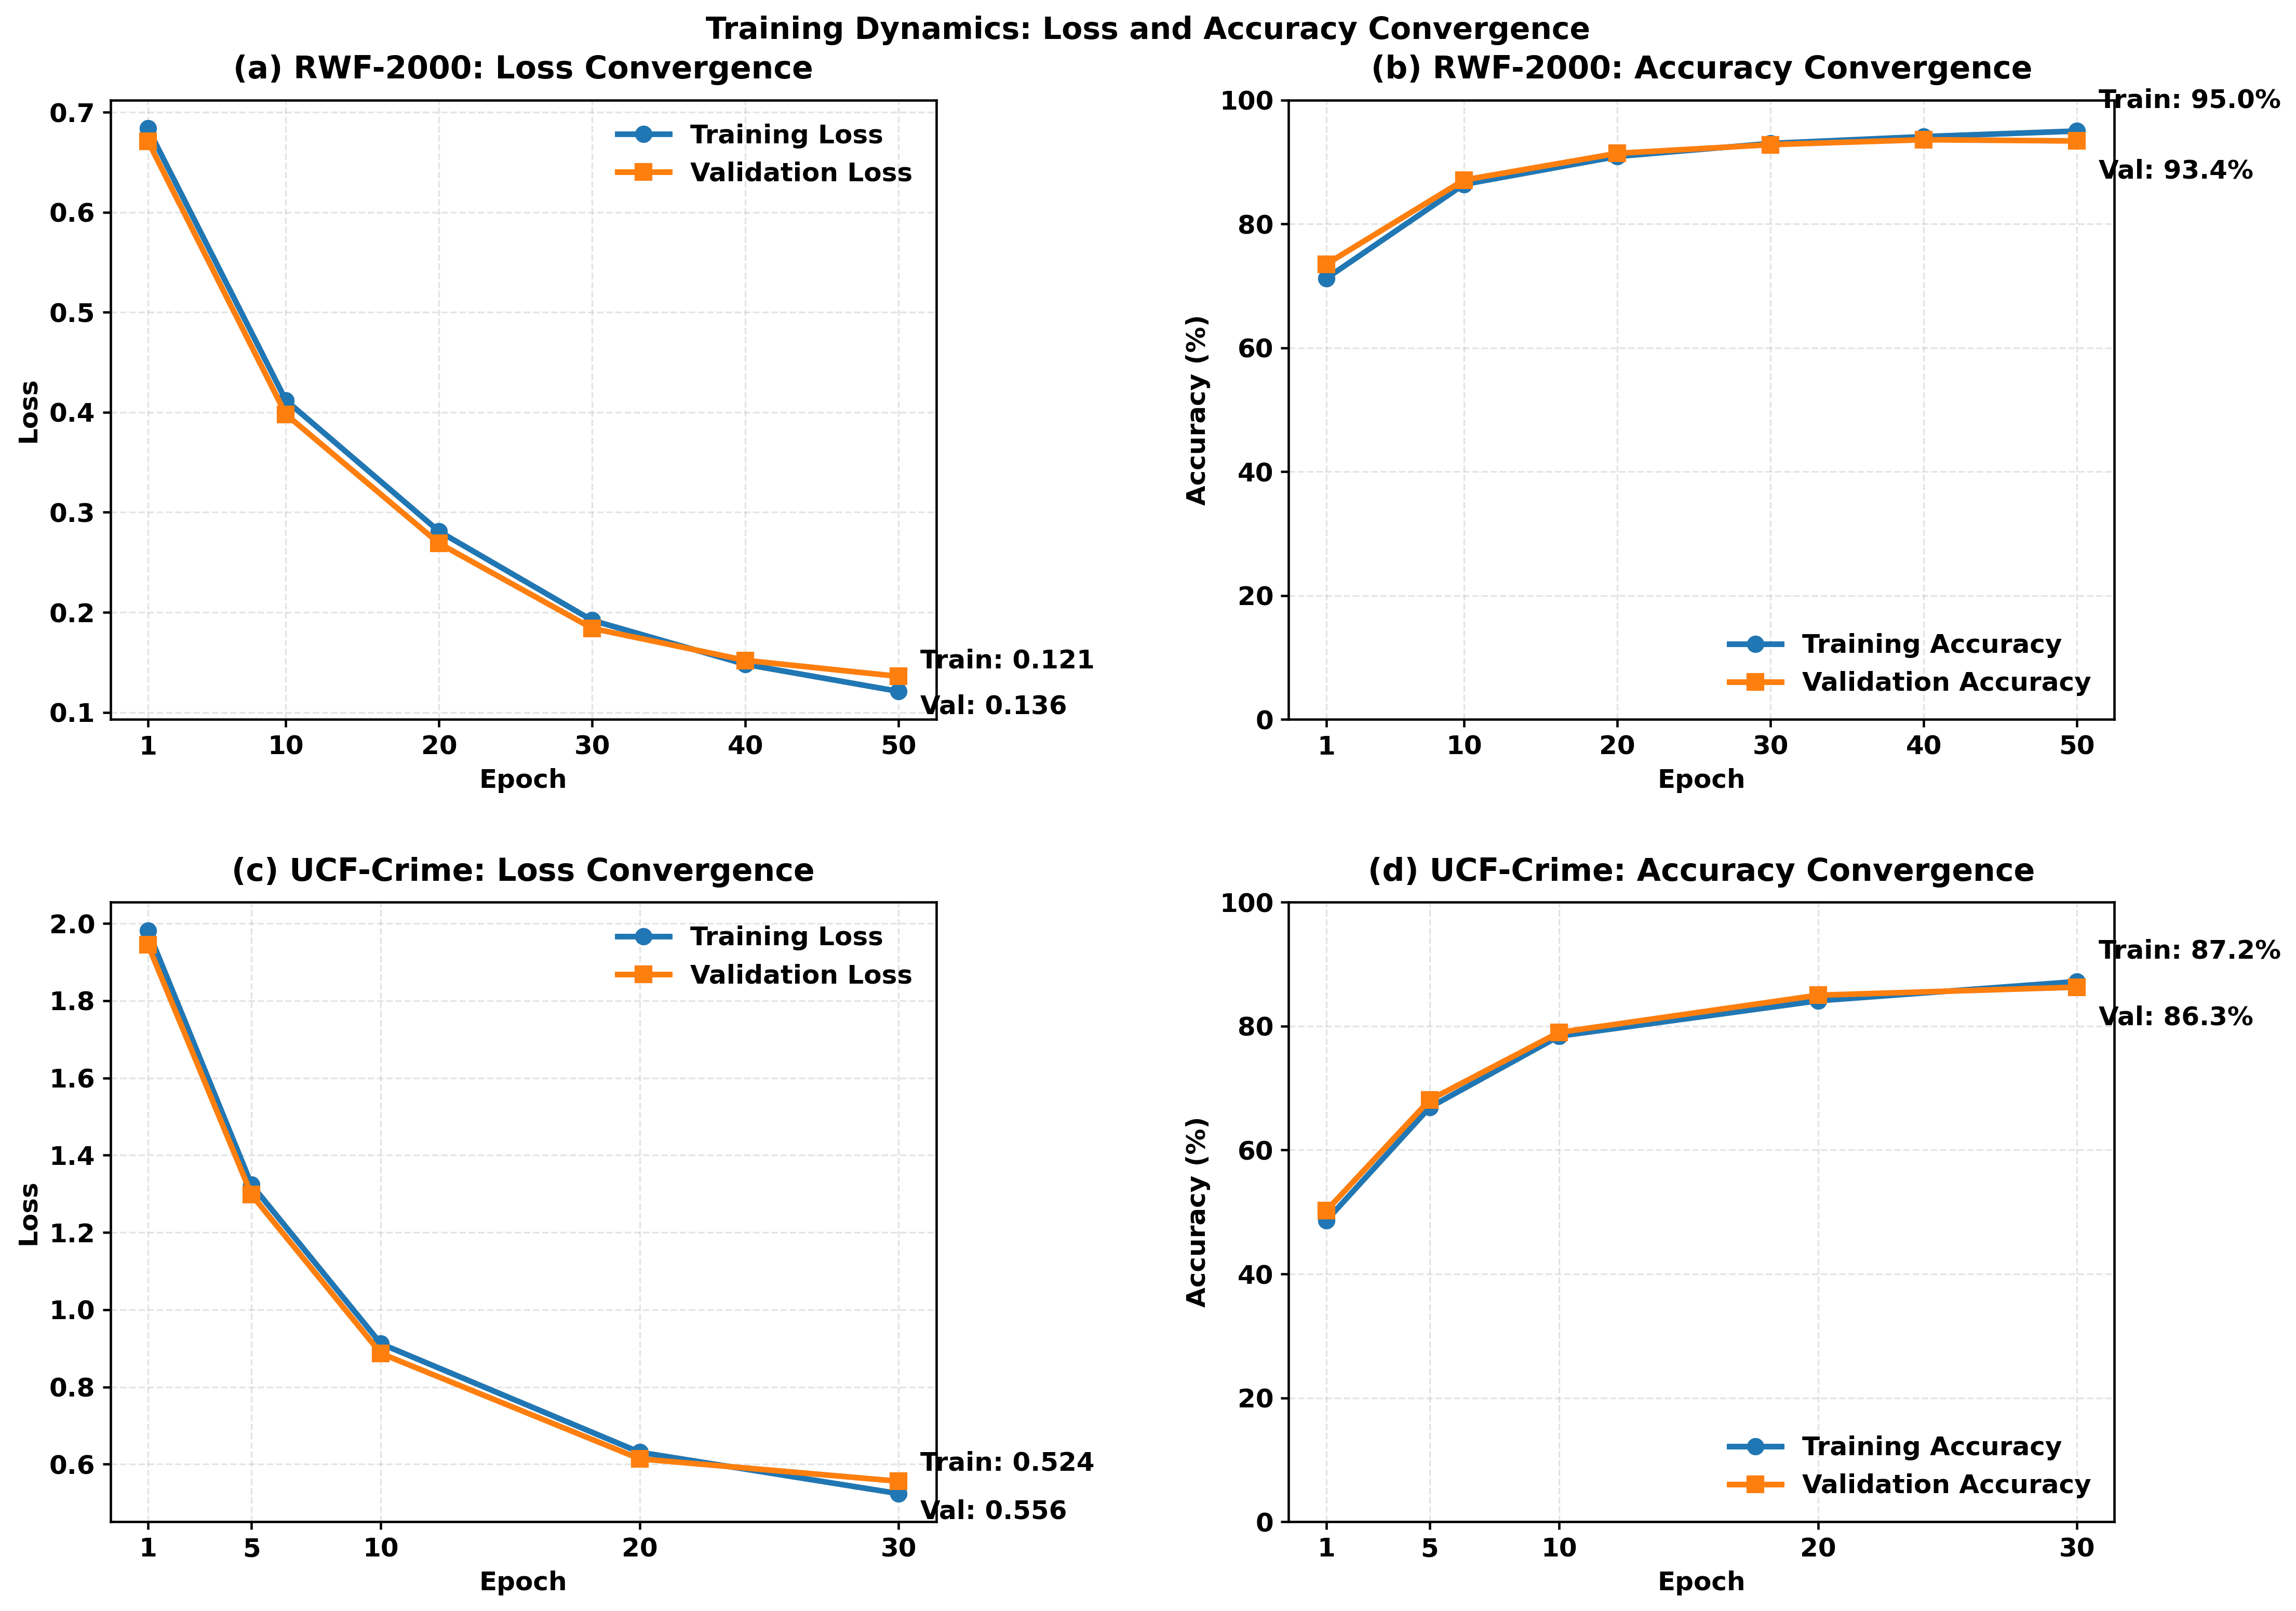
\includegraphics[width=0.9\linewidth]{7.png}
  \caption{Training loss and accuracy convergence on RWF-2000 and UCF-Crime.}
  \label{fig:training_dynamics}
\end{figure}


\subsection{Confusion Matrix Analysis on UCF-Crime}
To examine error structure beyond aggregate metrics, we report the row-normalized confusion matrix for EO-HTN on UCF-Crime in Table~\ref{tab:ucfcrime_cm}. The diagonal entries indicate class-wise recall, and several patterns are informative for surveillance deployment. The model shows strong separation for visually distinctive events. Normal is recognized with 92.4\% correct predictions, and Road Accident reaches 85.8\% on the diagonal, while Explosion and Shooting achieve 84.7\% and 82.1\%, respectively, suggesting that abrupt motion and context cues help reduce ambiguity in these categories. Some confusions are concentrated among semantically related human-interaction threats. Fighting is correctly classified at 84.1\%, but it is misclassified as Assault in 6.9\% of cases, and Assault is correctly classified at 81.6\% while shifting to Fighting at 7.8\%, reflecting overlap in close-contact motion patterns. Property-related threats show a similar coupling. Robbery has an 80.2\% diagonal rate and is most often predicted as Burglary at 6.4\%, whereas Burglary has a 78.5\% diagonal and shifts to Robbery at 5.7\%, which is consistent with shared indoor contexts and partial occlusion. Fine-grained categories of theft are still hard, where Stealing has a high 77.4\% diagonal and is mistaken with Shoplifting with 8.3\%, while Shoplifting has a high 74.9\% diagonal and is mistaken with Stealing with 7.5\%. Vandalism has a diagonal of 76.3\% and a significant drift towards Abuse at 9.6\%, thus suggesting that visually aggressive gestures and scene disorder can be similar to interpersonal harm cues at the clip level. The most prominent safety-critical case of confusion is around Shooting, where 9.1\% of Shooting clips are predicted as Explosion and 4.6\% are predicted as Arson, which can happen when there are flashes, smoke, or chaotic motion in the frames. Arrest is known to be a case at 80.6\%, however, 4.9\% of the Arrest clips are predicted as being Normal, which hints to the fact that restraint or escort actions can appear benign without clear context. Overall, Table~\ref{tab:ucfcrime_cm} emphasizes that EO-HTN has a good recall for distinguishable event classes but residual errors accrue in pairs which share motion dynamics and scene semantics, offering concrete targets for future refinement such as class-aware temporal sampling or auxiliary object cues. There is a visual per class view of the row normalized confusion patterns can be found in Fig.~\ref{fig:ucfcrime_confusion_lines}


\begin{table*}[t]
\centering
\caption{Detailed confusion matrix (\%) for UCF-Crime using EO-HTN (row-normalized).}
\label{tab:ucfcrime_cm}
\renewcommand{\arraystretch}{1.05}
\setlength{\tabcolsep}{2.8pt}
\resizebox{\textwidth}{!}{%
\begin{tabular}{|p{2.2cm}|c|c|c|c|c|c|c|c|c|c|c|c|c|c|}
\hline
\textbf{True $\backslash$ Pred} & \textbf{Normal} & \textbf{Fight} & \textbf{Assault} & \textbf{Robbery} & \textbf{Stealing} & \textbf{Vandal} & \textbf{Shooting} & \textbf{Burglary} & \textbf{Explosion} & \textbf{Arson} & \textbf{Accident} & \textbf{Shoplift} & \textbf{Abuse} & \textbf{Arrest} \\
\hline
Normal & 92.4 & 1.2 & 0.8 & 0.6 & 0.9 & 1.1 & 0.0 & 0.7 & 0.0 & 0.0 & 1.6 & 0.4 & 0.2 & 0.1 \\
\hline
Fighting & 1.5 & 84.1 & 6.9 & 0.8 & 0.3 & 1.2 & 0.5 & 0.6 & 0.0 & 0.0 & 1.0 & 0.4 & 0.4 & 0.3 \\
\hline
Assault & 1.7 & 7.8 & 81.6 & 1.1 & 0.4 & 1.0 & 0.6 & 0.7 & 0.0 & 0.0 & 0.8 & 0.6 & 2.7 & 0.0 \\
\hline
Robbery & 1.1 & 0.9 & 1.2 & 80.2 & 4.3 & 0.6 & 0.5 & 6.4 & 0.0 & 0.0 & 0.8 & 2.5 & 1.5 & 0.0 \\
\hline
Stealing & 1.4 & 0.6 & 0.7 & 3.9 & 77.4 & 0.9 & 0.2 & 2.8 & 0.0 & 0.0 & 0.7 & 8.3 & 3.1 & 0.0 \\
\hline
Vandalism & 2.1 & 0.7 & 0.9 & 0.8 & 1.0 & 76.3 & 0.3 & 5.1 & 0.0 & 0.0 & 2.4 & 0.8 & 9.6 & 0.0 \\
\hline
Shooting & 0.3 & 0.5 & 0.6 & 0.4 & 0.1 & 0.3 & 82.1 & 0.6 & 9.1 & 4.6 & 0.8 & 0.0 & 0.5 & 0.1 \\
\hline
Burglary & 1.6 & 0.8 & 0.9 & 5.7 & 2.4 & 2.1 & 0.4 & 78.5 & 0.0 & 0.0 & 0.7 & 4.6 & 2.3 & 0.0 \\
\hline
Explosion & 0.2 & 0.0 & 0.0 & 0.0 & 0.0 & 0.0 & 6.8 & 0.0 & 84.7 & 4.2 & 3.6 & 0.0 & 0.3 & 0.2 \\
\hline
Arson & 0.4 & 0.0 & 0.0 & 0.0 & 0.0 & 0.0 & 4.6 & 0.0 & 6.1 & 79.3 & 8.8 & 0.0 & 0.6 & 0.2 \\
\hline
Road Accident & 1.2 & 0.4 & 0.3 & 0.2 & 0.2 & 0.8 & 0.9 & 0.5 & 3.1 & 6.6 & 85.8 & 0.0 & 0.0 & 0.0 \\
\hline
Shoplifting & 1.8 & 0.5 & 0.6 & 2.7 & 7.5 & 0.9 & 0.0 & 2.1 & 0.0 & 0.0 & 0.9 & 74.9 & 8.1 & 0.0 \\
\hline
Abuse & 1.9 & 1.1 & 5.4 & 1.2 & 1.3 & 3.7 & 0.4 & 1.8 & 0.0 & 0.0 & 0.6 & 2.0 & 77.0 & 3.6 \\
\hline
Arrest & 4.9 & 0.6 & 0.4 & 0.3 & 0.2 & 0.5 & 0.1 & 0.4 & 0.0 & 0.0 & 0.3 & 0.2 & 0.1 & 80.6 \\
\hline
\end{tabular}%
}
\end{table*}

% ---------------- Figure 8 ----------------
\begin{figure*}[!t]
  \centering
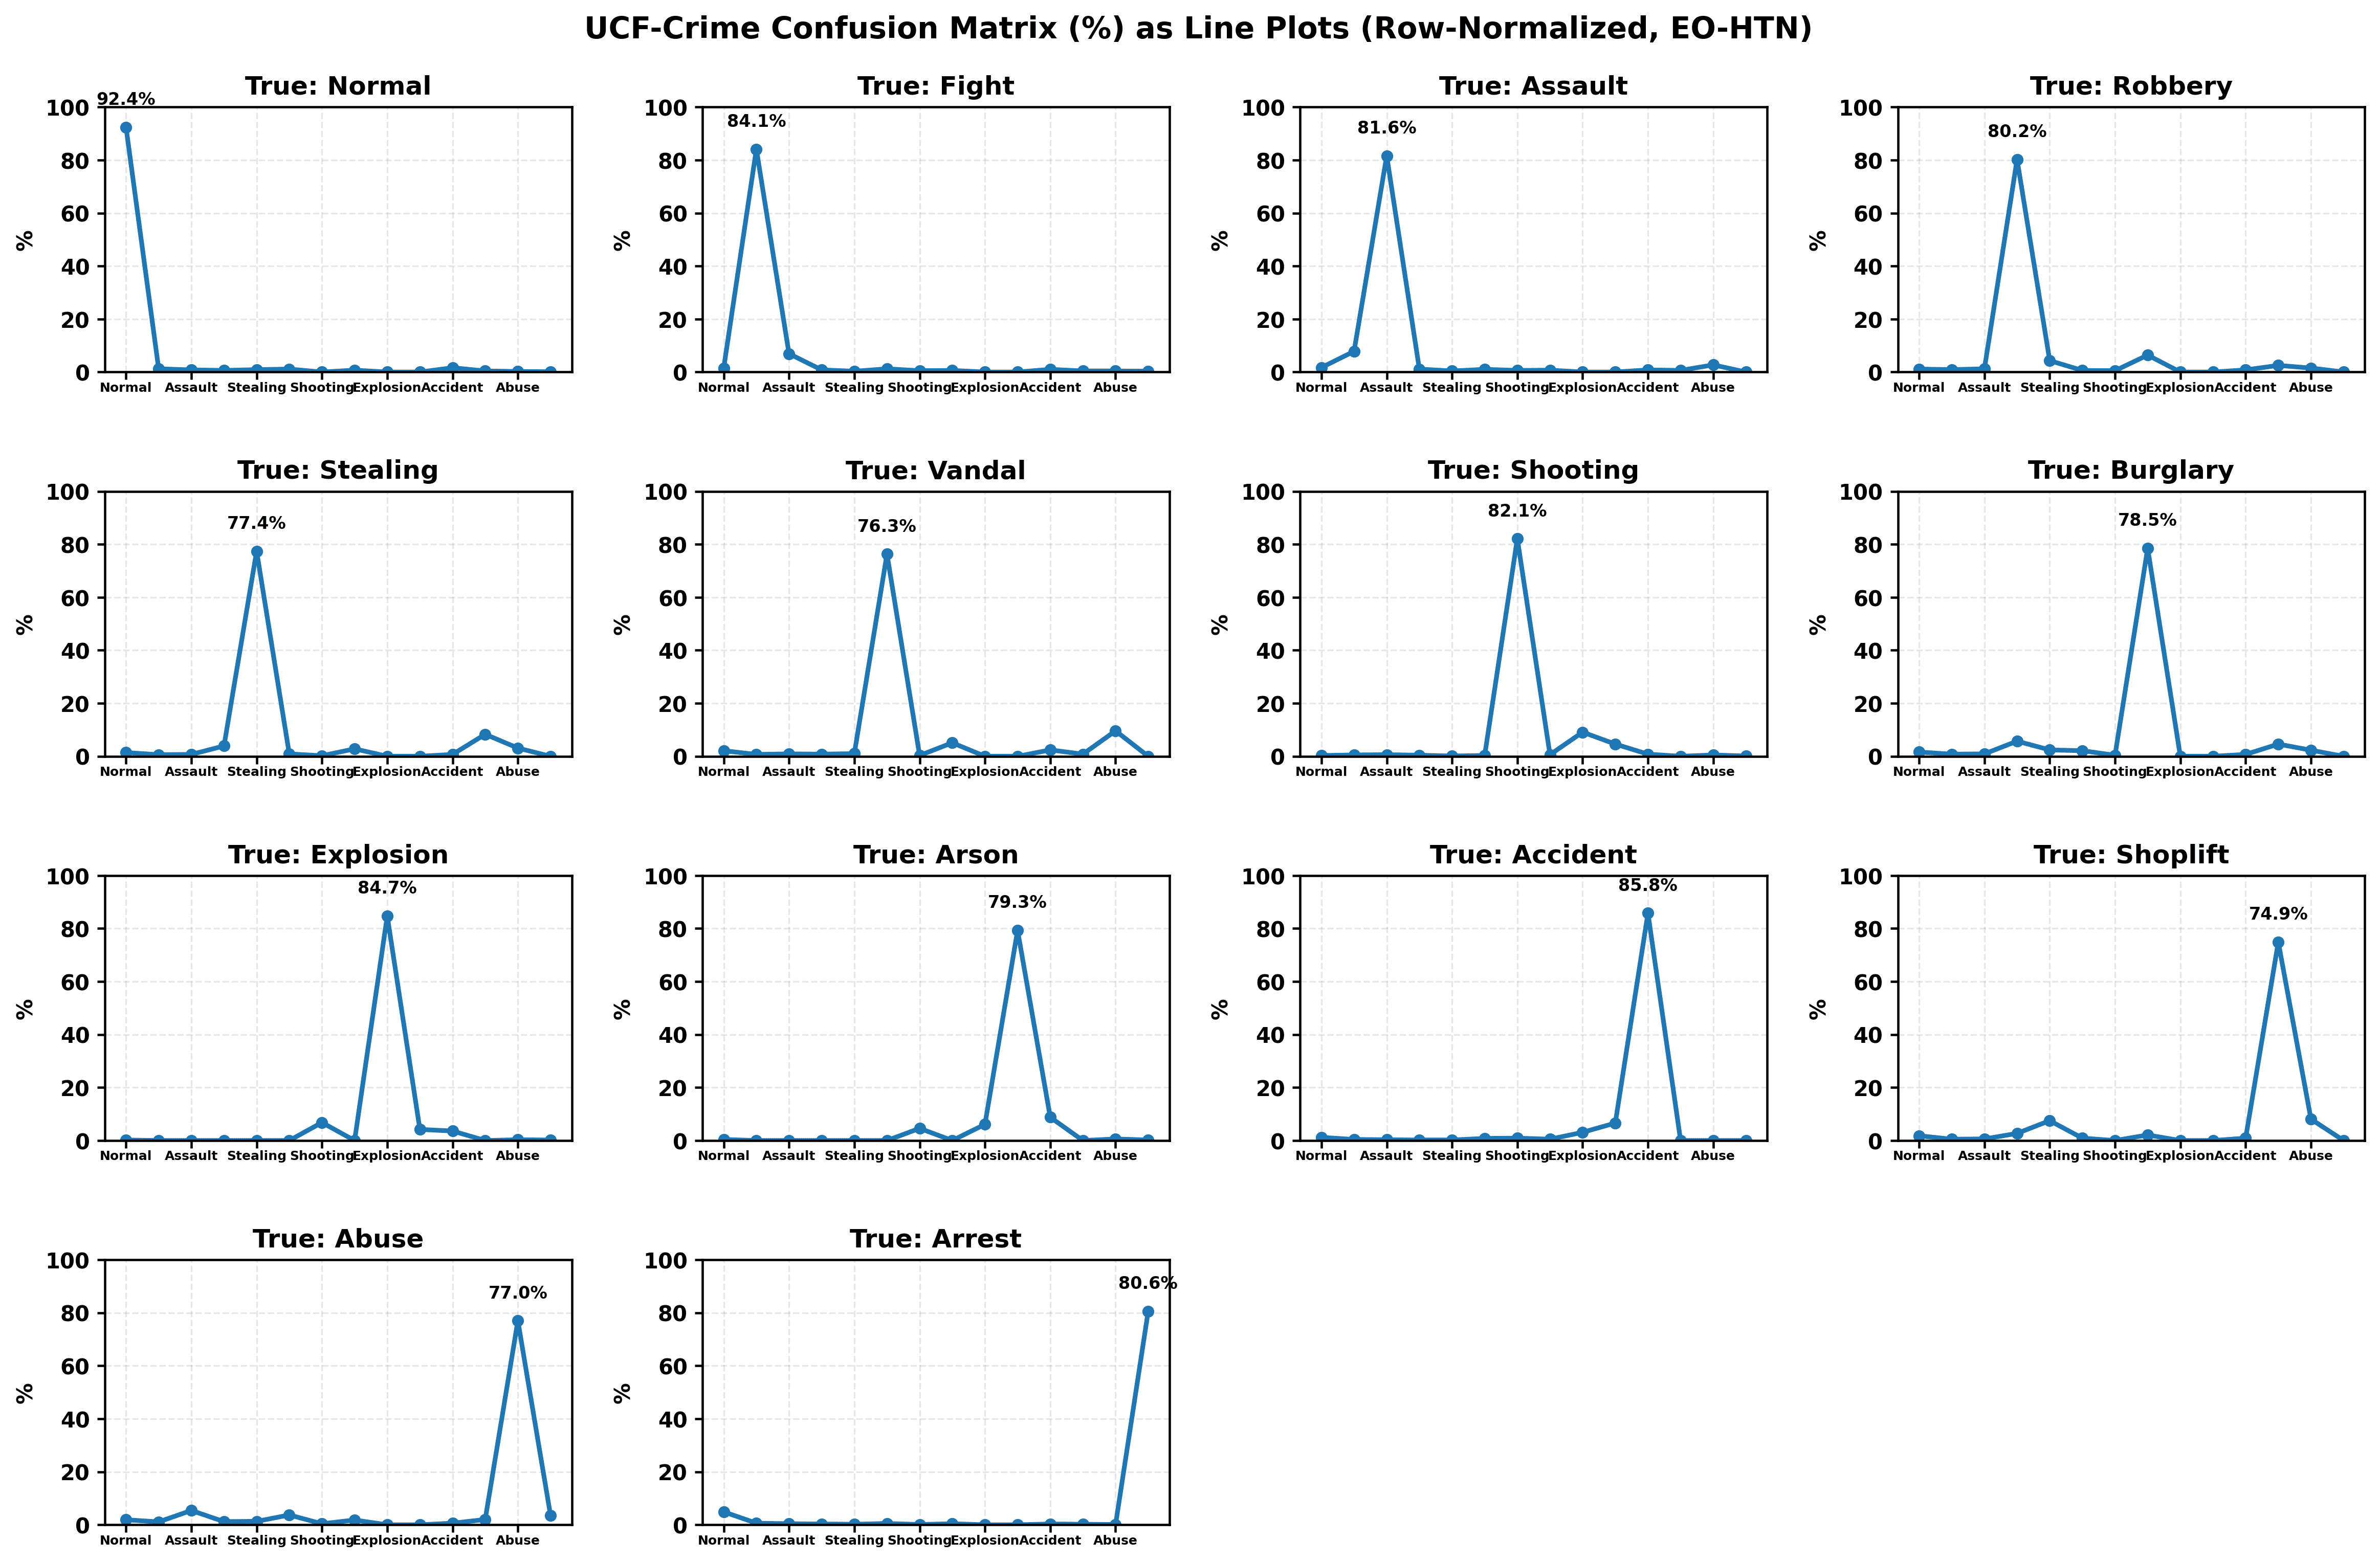
\includegraphics[width=0.9\linewidth]{8.png}
  \caption{UCF-Crime confusion matrix (\%) shown as per-class line plots (EO-HTN).}
  \label{fig:ucfcrime_confusion_lines}
\end{figure*}


\subsection{Calibration and Reliability on RWF-2000}
In surveillance threat classification, probability quality matters because downstream actions often depend on confidence thresholds rather than class labels alone. We therefore evaluate calibration on RWF-2000 using Brier score, expected calibration error (ECE), maximum calibration error (MCE), and negative log-likelihood (NLL), alongside accuracy. Table~\ref{tab:calibration_rwf2000} shows that EO-HTN achieves the best overall reliability profile while also delivering the highest accuracy. Specifically, EO-HTN reaches 93.4\% accuracy with a Brier score of 0.078, ECE of 3.2\%, MCE of 8.6\%, and NLL of 0.268. Compared to Video Swin-T, which attains 92.0\% accuracy with Brier score 0.091, ECE 4.1\%, MCE 10.2\%, and NLL 0.302, EO-HTN reduces calibration error and improves likelihood-based confidence quality. The trend is consistent against convolutional baselines. SlowFast (R50) records 90.3\% accuracy with Brier score 0.104, ECE 5.4\%, MCE 12.6\%, and NLL 0.351, while I3D reports 88.4\% accuracy with Brier score 0.118, ECE 6.2\%, MCE 14.8\%, and NLL 0.392. Overall, the results in Table~\ref{tab:calibration_rwf2000} indicate that EO-HTN not only improves classification correctness, but also produces probability estimates that better align with empirical outcomes, which is beneficial when the system must trade off missed detections and false alarms through operating-point selection.

\begin{table}[t]
\centering
\caption{Calibration and reliability comparison on RWF-2000.}
\label{tab:calibration_rwf2000}
\renewcommand{\arraystretch}{1.1}
\setlength{\tabcolsep}{3.8pt}
\begin{tabular}{|p{3.8cm}|c|c|c|c|c|}
\hline
\textbf{Model} & \textbf{Acc (\%)} & \textbf{Brier} $\downarrow$ & \textbf{ECE (\%)} $\downarrow$ & \textbf{MCE (\%)} $\downarrow$ & \textbf{NLL} $\downarrow$ \\
\hline
I3D & 88.4 & 0.118 & 6.2 & 14.8 & 0.392 \\
\hline
SlowFast (R50) & 90.3 & 0.104 & 5.4 & 12.6 & 0.351 \\
\hline
Video Swin-T & 92.0 & 0.091 & 4.1 & 10.2 & 0.302 \\
\hline
EO-HTN (Proposed) & 93.4 & 0.078 & 3.2 & 8.6 & 0.268 \\
\hline
\end{tabular}%
\end{table}





\subsection{Discussion}
The results collectively indicate that EO-HTN improves threat recognition while staying compatible with edge constraints, and the gains are consistent across binary and multi-class settings. On RWF-2000, EO-HTN reaches 93.4\% accuracy with a 93.4\% F1-score, exceeding Video Swin-T at 92.0\% accuracy and 91.7\% F1, while using far fewer parameters (7.4M versus 28.2M) and substantially lower compute (10.9 GFLOPs/clip versus 88.1 GFLOPs/clip). The ablation study supports a coherent explanation for this gap: moving from the CNN baseline (90.8\% accuracy, 90.7\% F1) to the hybrid base (91.8\%, 91.7\%) shows that compact attention improves short-clip temporal reasoning, and enabling context-aware adaptation lifts performance further to 92.7\% accuracy and 92.6\% F1, suggesting that scene-conditioned gating reduces false triggers from fast motion and crowd interactions. Distillation yields the full 93.4\% and the INT8 variant retains 93.1\% with a large deployment benefit. On UCF-Crime (clip-level), EO-HTN achieves 86.3\% Top-1 accuracy and 83.2\% Macro F1, outperforming Video Swin-T at 84.1\% Top-1 and 80.6\% Macro F1, and the class-wise profile shows strongest reliability for Normal (93.5\% accuracy, 92.4\% recall) and visually distinctive events such as Explosion (89.6\% accuracy, 84.7\% recall) and Road Accident (90.2\% accuracy, 85.8\% recall). Errors concentrate where semantics and motion overlap, including Fighting and Assault (6.9\% and 7.8\% cross-confusions) and Stealing and Shoplifting (8.3\% and 7.5\% cross-confusions), which aligns with the expected ambiguity of short clip segments sampled from untrimmed videos. Robustness tests reinforce practical value, since EO-HTN degrades less under low light (82.0\% accuracy, 78.1\% Macro F1) and motion blur (80.7\%, 76.9\%) than Video Swin-T (78.2\%, 73.4\%) and (76.9\%, 72.1\%), and repeated runs show stable gains with small variation, for example 93.4$\pm$0.2\% on RWF-2000 and 86.3$\pm$0.3\% on UCF-Crime. Calibration metrics further strengthen the case for operational use, since EO-HTN achieves lower uncertainty error on RWF-2000 with a Brier score of 0.078, ECE of 3.2\%, MCE of 8.6\%, and NLL of 0.268 compared with Video Swin-T at 0.091, 4.1\%, 10.2\%, and 0.302, indicating confidence scores that better reflect true correctness for threshold-based alerting.

From an application perspective, the combination of accuracy, robustness, and calibrated confidence supports several visual security workflows, including real-time violence warning in public spaces, monitoring of high-risk zones such as corridors and entry points, and triage systems that rank clips for rapid review by security staff. Edge measurements prove feasible in these settings On Jetson Orin Nano, EO-HTN achieves 45.5 FPS of FP32 while 22 ms/clip latency, and the INT8 deployment improves the throughput to 62.5 FPS while 16 ms/clip latency and reduces the model from 28 MB to 9 MB, which supports multi-camera streaming or higher frame rate processing under memory limitation. On Jetson Nano, for example, the INT8 gets the throughput from 18.5 FPS to 26.3 FPS, which can be important where power and compute budgets are tight. Despite these strengths, there are still limitations. The confusion matrix shows that there are still structured confusions between some safety-critical categories, for example, Shooting is incorrectly classified as Explosion (9.1\%) or Arson (4.6\%), and Arrest is incorrectly classified as Normal (4.9\%), and this could be problematic in high-stake deployments. Cross-dataset transfer also reveals a disparity when learning on a binary dataset from short clips and when attempting to transfer learning to a multi-class dataset, where accuracy falls to 81.6\% on the UCF-Crime Fight/Assault subset, which indicates that it is sensitive to dataset-specific context even when motion patterns are related. Clip-level protocols on untrimmed videos are still an approximation as threats may be sparse and temporal boundaries may not match sampled clips and performance in continuous streams may be dependent on the clip sampling strategy and alert aggregation. Future improvements could be focusing on reducing the structured confusions through class-aware sampling, auxiliary cues for objects and interactions, and better temporal aggregation for untrimmed inference, while preserving the compact design for reliable edge deployment.



\section{Conclusion}
This study demonstrates that the Edge-Optimized Hybrid Transformer Network with Context-Aware Adaptation (EO-HTN) can deliver strong threat recognition accuracy while remaining suitable for edge deployment in visual security systems. On RWF-2000, EO-HTN achieves 93.4\% accuracy with a 93.4\% F1-score, and on UCF-Crime under a clip-level protocol it attains 86.3\% Top-1 accuracy with an 83.2\% Macro F1-score, while maintaining a compact footprint of 7.4 million parameters and 10.9 GFLOPs per clip. Deployment measurements further support practical use, where inference on Jetson Orin Nano reaches 45.5 FPS in FP32 and 62.5 FPS after INT8 quantization, alongside a reduction in model size from 28 MB to 9 MB, enabling real-time monitoring for applications such as violence alerting, anomaly triage, and incident indexing in multi-camera environments. Despite these strengths, residual confusions persist among visually similar categories, and cross-dataset transfer remains challenging, as indicated by a drop to 81.6\% accuracy when training on RWF-2000 and testing on the UCF-Crime Fight/Assault subset, which suggests sensitivity to dataset-specific context and clip sampling. Future work should focus on reducing structured confusions using class-aware temporal sampling and auxiliary interaction cues, extending evaluation to streaming untrimmed inference with alarm aggregation, and improving robustness to domain shifts through adaptation or self-supervised pretraining while preserving the efficiency that makes edge deployment feasible.











\bmsection*{Data Availability}
The data supporting the findings of this study are available from the corresponding author upon reasonable request. All relevant datasets have been anonymized to protect participant confidentiality. No proprietary or restricted-access data were used in this research.


\bmsection*{Financial disclosure}
No funding was used in this study.

\bmsection*{Conflict of interest}
The authors declare no potential conflict of interests.

% Bibliography: keep as-is; undefined citations produce warnings, not errors.
\bibliography{wileyNJD-APA}



\end{document}
